\documentclass[twoside]{dis04}
\usepackage{epsfig}
%\def\runauthor{Kamil Sedl\'{a}k}
\def\runauthor{PSI}
% for the H1 collaboration}
\def\shorttitle{musrSim}
\begin{document}

%\newcommand{\xgmy}{\ensuremath{x^{\mathrm{jets}}_\gamma} }
%\newcommand{\GeV}{\ensuremath{\mathrm{GeV}} }
%\newcommand{\pb}{\ensuremath{\mathrm{pb}} }
%\newcommand{\gevsq}{\ensuremath{\mathrm{GeV}^2} }
%\newcommand{\Etone}{\ensuremath{E^*_{T\, 1}} }
%\newcommand{\Ettwo}{\ensuremath{E^*_{T\, 2}} }
%\newcommand{\Etmy}{\ensuremath{E^*_T} }
%\newcommand{\etaone}{\ensuremath{\eta^*_{1}} }
%\newcommand{\etatwo}{\ensuremath{\eta^*_{2}} }
%\newcommand{\etamy}{\ensuremath{\eta^*} }
%\newcommand{\ycut}{\ensuremath{y_c} }
\newcommand{\musr}{\ensuremath{\mu}SR}

\title{Manual of musrSim}
%\title{GEANT Simulation Program for the
%$\mathbf{\mu}$SR Instruments}

\author{Kamil Sedl\'ak$^1$, Toni Shiroka$^1$, Zaher Salman$^1$, Jose Rodriguez$^1$, Tom Lancaster$^2$, Thomas Prokscha$^1$, Taofiq Para\"{\i}so$^1$, Robert Scheuermann$^1$, James S. Lord$^3$}

\address{{$^1$ Laboratory for Muon Spin Spectroscopy, Paul Scherrer Institut, CH-5232 Villigen PSI, Switzerland}\\
$^2$ Clarendon Laboratory, Department of Physics, Oxford University, Parks Road, Oxford OX1 3PU, UK\\
$^3$ ISIS Facility, Rutherford Appleton Laboratory, Chilton, Oxon OX11 0QX, U.K.}
%\address{{\rm (on behalf of the H1 collaboration)}\\
%Institute of Physics AS\,CR\\
%%Academy of Sciences of the Czech Republic
%Na Slovance 2, 182 21 Praha 8, Czech Republic\\
%E-mail: ksedlak@fzu.cz}

\maketitle
\footnotesize
\begin{center}
  PSI, August 12th, 2016
\end{center}\vspace{2mm}
\normalsize
\abstracts{
``musrSim'' is a simulation program based on Geant4,
optimised for the $\mu$SR instruments.
This document describes some of the commands used in the user macros
of the simulation program for the $\mu$SR instruments based on the {\sc
Geant4}. The root output variables are also described.}

%========================================================================================================
\section{Scope of the musrSim program}
The program ``musrSim'' is a relatively general program that can be used to simulate 
the response of a $\mu$SR~\cite{Blundel:1999} instruments (detectors) to muons and their decay particles 
(electrons, positrons and gammas), optionally including ``optical photons''.
Even though musrSim is tailored to the needs of 
the $\mu$SR technique~\cite{shirokaGeant}, it has been used also 
in the studies of beam-line elements like spin rotators, as well as
in the detector development
studies without any muons involved, e.g.\ to test the response of an APD-based 
scintillator counters to the irradiation of Sr radioactive source~\cite{FirstExperience}.
It should be straightforward to apply musrSim also to the low energy particle-physics
experiments with muons.

The program is based on the Geant4~\cite{geant} and Root~\cite{root} libraries.
Geant4 is Monte Carlo toolkit used (not only) in particle physics to simulate
the passage of particles through detectors.
Root is an analysis tool that allows one to manipulate and analyse the simulated data, 
namely to plot histograms and other graphical output.

The simulation of an instrument consists of two steps -- simulation of the instrument
response, which is done by ``musrSim'' program, and the subsequent analysis of the
simulated output by either ``musrSimAna'' program (in case of \musr instruments) or
by Root (if a special analysis is required, e.g.\ for non-\musr apparatus).
The reason for this spit is purely
practical -- while it takes a lot of computer time to simulate large statistics data
with musrSim, the subsequent analysis of the simulated data is relatively quick
and allows the user to optimise and test different options of the analysis 
(e.g.\ different thresholds in positron counters, different logic in connecting 
veto and coincidence detectors, different rate of incoming muons, ...).
The ``musrSimAna'' program is described in a separate manual.

The aim of the musrSim is to provide an easy-to-use simulation program, which does
not require a deep knowledge of Geant4 in order to simulate a ($\mu$SR) detector.
In our view, the main advantages of musrSim are:
\begin{itemize}
	\item Simple way how to define or modify the instrument geometry, including
	      the sample environment, collimators and other parts.
	\item Limited (ideally no) need to modify and/or recompile the source code,
	      because the parameters defining the instrument geometry, initial muon beam,
	      electromagnetic fields, and other parameters are defined in
	      a text file (the so called ``macro file'').
	\item Implementation of the  $\mu$SR-specific classes (muon spin rotation
	      in magnetic fields, muonium formation and decay, ...).
	\item Possibility to read in the output files of the TURTLE~\cite{turtle}
	      program for the beam-line simulation.
	\item Simple way how to define (overlapping) electromagnetic fields.
	\item Output in the Root tree.
	\item Possibility to analyse the output with a general ``musrSimAna'' program.
	\item Possibility to use musrSim easily for calculating muon stopping profile 
	      (also in e.g.\ sample cells) or in developments of detector components
	      (e.g.\ light propagation in the scintillator of a positron/muon counter
	      and the subsequent light collection in a photomultiplier tube or APD).
\end{itemize}
%
On the other hand, there are also some drawbacks and limitations:
\begin{itemize}
	\item The user has to have an installation of Geant4 and Root before installing musrSim. 
	\item It is supposed the user will analyse the data with Root, therefore
	      Root has to be installed.
	\item At present time the program does not simulate any muon-spin related
              physics processes happening in the sample, except for the muon 
              spin rotation.
	\item The simulation of one event takes much more time than the measurement
	      of a real event. The simulation time depends on the
	      complexity of the instrument geometry and on the presence of
	      electromagnetic fields.  To simulate one million of muons
	      in the case of the PSI high-field instrument took about 10 hours
	      of a computer time of a desktop PC.
\end{itemize}

%=============================================================================================
\section{How to install and run musrSim}
To install and run musrSim, one has to install Geant4 and Root first.
The present version of musrSim has been tested with Geant version 4.9.4,
and with Root version 5.24.00. While the version of Root should not be critical,
the users of musrSim are encouraged to always use the latest version of Geant4
due to continuous improvements of this package. A novice
user of Geant4 may consider reading 30 pages of chapter~2 of the 
Geant4 User's Guide for Application Developers, called 
``Getting Started with Geant4 - Running a Simple Example''.

Once Geant4 has been successfully installed and some of the default Geant4 examples
has been run, the musrSim installation package can be downloaded from the web page 
http://lmu.web.psi.ch/simulation/index.html.
Usually the ``env.sh'' script has to be run to set-up the environment variables
appropriately before the musrSim (and/or any other Geant4 application) can be compiled
and run.
The simulation is started by executing: 

{\bf $>$ musrSim \emph{RUNNUMBER}.mac} \\
where \emph{RUNNUMBER}.mac is a ``macro file'' containing the information about 
the instrument setup.  The string \emph{RUNNUMBER} is an integer representing the run number.

In order to simulate a new instrument, the user has to define the following blocks of information
in the macro file:
%
\begin{itemize}
	\item Define the geometry (the so-called ``volumes'') of the new instrument.
	Note that in Geant4 volumes can be included inside other volumes 
	(a ``daughter'' volume is positioned inside its ``mother'' volume),
	and it is therefore necessary to distinguish between the global (world)
	coordinates and the coordinates of the daughter volumes (local coordinates).
	It is not allowed to overlap the volumes (with the exception of the 
	daughter and mother volume, in which case the daughter volume has to be fully
	contained within its mother volume).
	\item Define the electric and magnetic fields.
	\item Define physics processes relevant for your case.
	\item Define the initial muon parameters (more generally -- initial particle parameters).
	\item Define some other parameters influencing the execution of the simulation.
	\item Define which variables should be written out to the output Root tree.
	\item In case it is required to visualise the geometry, define the visualisation attributes.
\end{itemize}

By default, the output of the simulation is written out in the subdirectory ``data'' with
the name ``musr\_RUNNUMBER.root''.  The default ``data'' subdirectory can be changed 
(see Chapter~\ref{sec:otherParameters}).  The simulated data are stored in a Root tree,
which is some kind of a table with many variables for every simulated event, inside
the musr\_RUNNUMBER.root file.


%%%%%%%%%%%%%%%%%%%%%%%%%%%%%%%%%%%%%%%%%%%%%%%%%%%%%%%%%%%%%%%%%%%%%%%%%%%%%%%%%%%%%%%%%%%%%%%%%%
\section{How to stop musrSim}
The execution of musrSim stops as soon as one of the following condition is fulfilled:
\begin{itemize}
	\item Number of simulated events reaches the number of required events defined by
	  command ``{\bf /run/beamOn \emph{nrOfEvents}}'' (see Chapter~\ref{sec:otherParameters}).
	\item Time for which the simulation is running exceeds the maximum allowed time defined
	  by command ``{\bf /musr/command maximumRunTimeAllowed \emph{timeMax}}''
	  (see Chapter~\ref{sec:otherParameters}).
	\item Within a few seconds after a file ``RUNNUMBER.stop'' is created in the
	  directory, in which the musrSim program was started.  This allows the user
	  to stop the simulation gently at any time.
\end{itemize}
If the musrSim program is killed in any other way, the output Root file does not close properly, and
subsequently can not be analysed.  The simulated data are lost.
%%%%%%%%%%%%%%%%%%%%%%%%%%%%%%%%%%%%%%%%%%%%%%%%%%%%%%%%%%%%%%%%%%%%%%%%%%%%%%%%%%%%%%%%%%%%%%%%%%
\section{Conventions}
The default units of the musrSim in both the macro file (RUNNUMBER.mac) and in the Root tree 
are summarised in table~\ref{tab:units}.
\begin{table}[htb]\centering
\renewcommand{\arraystretch}{1.05}
  \begin{tabular}{lp{5mm}l}
    \hline
    \lower 1mm \hbox{\textbf{Quantity}}  &&  \lower 1mm \hbox{\textbf{Default unit}} \\[5pt]
    \hline
     Length      &&  mm  \\
     Time        &&  $\mu$s (sometimes ns) \\
     Energy      &&  MeV \\
     Momentum    &&  MeV/c\\
     Magnetic field   && tesla \\
     Electric field   && keV/mm \\
     Angle           && degree \\
     \hline
  \end{tabular}
  \caption{The default units of musrSim.}
  \label{tab:units}
\end{table}
%%%%%%%%%%%%%%%%%%%%%%%%%%%%%%%%%%%%%%%%%%%%%%%%%%%%%%%%%%%%%%%%%%%%%%%%%%%%%%%%%%%%%%%%%%%%%%%%%%
\section{Tips and tricks}
\begin{itemize}
  \item Visualise your instrument geometry during its construction.
  \item Check the output file for error messages, especially for volume overlaps.
  \item Note the the dimensions in volume definitions are often half-lengths, not
        the lengths (e.g.\ half-lengths of the box edges).
  \item The order of some commands in macro file matters -- e.g.\ one has to define
        a mother volume before the daughter volume, etc.
  \item There are some special volume names, namely \emph{World}, 
        \emph{Target}  (same as \emph{target}), \emph{M0}, \emph{M1}, \emph{M2} and
	volumes starting with keywords \emph{Shield} (same as \emph{shield}), and
	volumes containing string \emph{save}.  All these volume influence the
	behaviour of the simulation, so understand how they act (see different chapters
	of this manual) before you use them.
  \item When implementing a new magnetic or electric field always check that fields at
        a few random space points correspond to the field you expect to observe
        (use command /musr/command globalfield printFieldValueAtPoint~).
\end{itemize}
%%%%%%%%%%%%%%%%%%%%%%%%%%%%%%%%%%%%%%%%%%%%%%%%%%%%%%%%%%%%%%%%%%%%%%%%%%%%%%%%%%%%%%%%%%%%%%%%%%
\section{Detector construction}
The user must first define the instrument geometry in the macro file. It should be relatively
easy to understand how this is done from the example macro files distributed with musrSim
program.

An important parameter to note in the following description of ``/musr/command construct'' 
command is the \emph{idNumber} -- an integer number uniquely identifying every volume.  
The ID volume numbers are later on used also in the musrSimAna program, when some identification 
of a volume becomes necessary (i.e.\ volumes are described by \emph{idNumber} rather than
by their \emph{name} command later on).

Another crucial parameter in ``/musr/command construct'' command 
is \emph{sensitiveClass}, which defines whether the volume
is sensitive (i.e.\ a signal can be detected in the volume) or not (i.e.\ the volume
is just a dead material influencing the penetrating particles but not detecting them).
 
There are some special kind of volumes, which are defined by the name (or part of the name).
The user can (but does not have) to use them.
The first of them is the volume named ``Target'' (or ``target'').  It is expected, that
this is the sample, and the quantities {\tt muTargetTime, muTargetPolX, muTargetPolY, muTargetPolZ,
muTargetMomX, muTargetMomY, muTargetMomZ},
will be saved when a muon enters this volumes for the first time in a given event. 

The second special kind of volumes are the volumes named ``M0'', ``M1'' and ``M3'' (or ``m0'',
``m1'' and ``m3'').  Typically these volumes can be trigger detectors. 
The quantities  {\tt muM0Time, muM0PolX, muM0PolY, muM0PolZ} 
will be saved when a muon enters the volume called ``M0'' (or ``m0'')  for the first time
(similarly for ``M1'' and ``M2'').
Note that it is not expected that {\tt muM0Time} should be used in the analysis of the
simulation -- one should use the {\tt det\_time\_start} quantity, which corresponds
to the measured time in the experiment.

The third class of special volumes has names starting with the string ``save''.
Their purpose in the simulation is usually to check positions
and momenta of particles at some position of the detector, even if the particle does not deposit any energy in
the given ``save'' volume.  Save volumes can therefore be made of vacuum.
See section\ref{sec:rootVariables} for further details on what is saved in the Root tree.

The last special class of volumes has names starting with the string ``kill'',
``shield'' or ``Shield''.
If a particle enters the ``kill \ldots'' volume, it is removed from further simulation.
The same is true for the ``shield \ldots'' or ``Shield \ldots'' volumes for
any particle apart for a muon.
The motivation for this kind of volumes was to speed up the simulation by removing tracks
that are unlikely to hit any detector. The ``kill'', ``shield'' and ``Shield'' volumes should be use with
care.

\begin{description}

\item{\bf /musr/command construct \emph{solid} \emph{name} \emph{dimensions} ... \emph{material} 
	\emph{x} \emph{y} \emph{z} \emph{motherVolume} \emph{matrixName} 
	\emph{sensitiveClass} \emph{idNumber} }\\
	This command defines a volume in {\sc Geant4} (It comprises three steps of {\sc Geant4}: defines a solid,
        logical volume and physical volume.  Details can be found in {\sc Geant4} manual). \\
	\begin{itemize}
	\item \emph{solid} (string) can be one of the G4VSolid.cc particular types, presently ``tubs'', ``cons'',
	             ``box'', ``trd'', ``sphere'', ``para'', ``polycone''
	             or it can be one of the specifically implemented solids by our program as ``uprofile'' 
	             (an U-profiled bar), ``alcSupportPlate'' (shape specific to ALC support plate), ``tubsbox'' 
	             (a tube with a rectangular hole along its axis), ``tubsboxsegm'' 
	             (a volume that looks like an intersection of tube and box) and 
                     ``trd90y'' (a trd volume rotated by 90 degrees around $y$ axis in addition
                     to the rotation requested by \emph{matrixName}), 
		     ``cylpart'' (cylinder from which a box has been subtracted)
		     ``GPDcollimator'' (collimator used at GPD instrument).  Not all G4VSolids defined
		     in Geant4 are
                     presently supported, but it is relatively easy to implement a new kind of solids
                     in the musrDetectorConstruction.cc class.
		     
		     The ``polycone'' in Geant4 can be defined in two ways, which have to be 
		     distinguished in the musrSim macro file:
		     ``polyconeA'' corresponds to \\
		     G4Polycone(solidName, phiStart, phiTotal, numZPlanes, zPlane[ ], rInner[ ], rOuter[ ])\\
		     while  ``polyconeB'' corresponds to \\
		     G4Polycone(solidName, phiStart, phiTotal, numRZ, r[ ], z[ ]),\\
		     where \emph{zPlane}, \emph{rInner}, \emph{rOuter}, \emph{r}, \emph{z} are arrays, which
		     have to be defined by the command ``/musr/command arrayDef''.
	\item \emph{name} (string) stands for the name of the volume.  As the command 
		     ``/musr/command construct'' constructs
	             three kinds of Geant4 classes/volumes (the solid, logical volume and physical 
	             volume), there are three names of the concrete volume used internally inside 
                     musrSim: sol\_\emph{name}, log\_\emph{name} and phys\_\emph{name}.
	              The main volume, inside which all other volumes are positioned, has to be called  ``World''.
	\item \emph{dimensions} (floats) define the size of the required solid.  They are kept equivalent to the
	             dimensions of solids as used in {\sc Geant4}.  For example the ``box'' is defined
	             by its {\bf halflengths} along $x$, $y$ and $z$ coordinates.  Note that the number of
	             \emph{dimensions} varies for each type of solid.  The units are mm for lengths
		     and degrees for angles.
	\item \emph{material} (float) one of the materials defined in {\sc Geant4}, namely in the file 
	             \$G4INSTALL/source/materials/src/G4NistMaterialBuilder.cc (e.g. ``G4\_Galactic'' for
	             vacuum, ``G4\_Cu'' for copper, ``G4\_AIR'' for air, 
                     ``G4\_PLASTIC\_SC\_VINYLTOLUENE'' for a scintillator, ...).
	             One can also define a new material inside the function 
                     musrDetectorConstruction::DefineMaterials().  Presently ``Mylar'', ``Brass'' 
                     ``Steel'', ``Macor'', ``MCPglass'', ``MgO'', ``SiO2'', ``Al2O3'', ``K2O'' and ``B2O3'' are defined there.
	\item \emph{x, y, z} (floats) -- coordinates of the volume, used to position the volume within
                     its mother volume (as used by the G4PVPlacement).  
		     Thus these coordinates are interpreted in the local coordinate system of the \emph{motherVolume}.
	\item \emph{motherVolume} (string) -- name of the mother volume, in which the given volume should be
	             positioned.  Note that the mother volume has to be defined first (before its
                     daughter), and that the name of mother starts with a string {\bf log\_}\emph{mothername},
	             following the naming convention defined above.  
	             When the ``World'' volume is defined, its \emph{motherVolume} should be set to ``no\_logical\_volume''.
	\item \emph{matrixName} (string) -- name of the rotation matrix that will be used to position
	             the volume inside its mother volume (as used by the G4PVPlacement).  
	             Use string ``norot'' if no rotation is required for the given volume.
	             Otherwise the rotation matrix has to be defined by the command line 
	             ``/musr/command rotation'' {\bf before} the given volume is defined. 
        \item \emph{sensitiveClass} (string) -- specifies whether the volume is sensitive detector or
		     just a piece of a ``dead'' material.
	             Use the string ``dead'' for the latter,
	             and the string ``musr/ScintSD'' for a scintillator (a sensitive volume, i.e.\
                     a volume where hits are observed).  No other detector type
	             (other than ``dead'' and ``musr/ScintSD'') is supported at the moment, but
	             the program might be extended in the future (e.g. to properly include also the
	             semiconductor tracking detectors, etc.).
	\item \emph{idNumber} (int) -- serves as a unique identifier of the volume.  It is primarily
	             used in the output Root tree to identify the volume: 1) in which a muon stopped 
	             (tree variable ``muDecayDetID''), 
	             2) in which hits were deposited in case of sensitive volume 
                     (the variable ``det\_ID[det\_n]'').
	\end{itemize}	

\item{\bf /musr/command rotation \emph{matrixName} $\alpha$ $\beta$ $\gamma$} \\
	{\bf /musr/command rotation \emph{matrixName} \emph{vx} \emph{vy} \emph{vz} \emph{angle}}\\
	These commands define a rotation matrix of the name \emph{matrixName} that can be used
	during the definition of the detector geometry (see the command ``/musr/command construct'').
	It can be defined either by the Euler angles (if there are three float parameters behind the
        \emph{matrixName}) or by the vector \emph{(vx,vy,vz)} and an \emph{angle} of rotation around this
	vector (if the fourth float parameter behind the \emph{matrixName} is non-zero).
	All angles are specified in degrees.

\item{\bf /musr/command arrayDef \emph{arrayName} \emph{N} \emph{x$_1$} \emph{x$_2$} \ldots \emph{x$_N$}} \\
        Defines an array with an assigned name \emph{arrayName}, which has \emph{N} elements.

\item{\bf /musr/command region define  \emph{regionName} \emph{logicalVolume}}\\
	The ``G4Region'' can be created using this command, and a logical volume of the
	name \emph{logicalVolume} will be assigned to it.  If the G4Region of the name 
	\emph{regionName} does not exist (i.e.\ the command ``/musr/command region define''
	is called for the first time for this particular \emph{regionName}), the G4Region will
	be created first, otherwise the logical volume \emph{logicalVolume} will be just assigned
	to the already existing G4Region.  \\
	G4Region can be useful namely for setting some special Geant4 parameters (production cuts)
	just in some part of the detector (e.g.\ where a finer simulation is needed).
	See Geant4 manual for more details.

\item{\bf /musr/command region setProductionCut \emph{regionName} \emph{gammaCut} \emph{electronCut} \emph{positronCut}}\\
	Set the so-called ``production cuts'' in the G4Region called \emph{regionName}.
	The variables \emph{gammaCut, electronCut} and \emph{positronCut} are given in mm.
\end{description}


%%%%%%%%%%%%%%%%%%%%%%%%%%%%%%%%%%%%%%%%%%%%%%%%%%%%%%%%%%%%%%%%%%%%%%%%%%%%%%%%%%%%%%%%%%%%%%%%%%
\section{Electric and magnetic fields}
\begin{description}
\item{\bf /musr/command globalfield \emph{fieldName} \emph{half\_x} \emph{half\_y} \emph{half\_z} uniform 
	\emph{X} \emph{Y} \emph{Z} \emph{logicalVolume} \emph{Bx} \emph{By} \emph{Bz} \emph{Ex} \emph{Ey} \emph{Ez}} \\
	or \\
	{\bf /musr/command globalfield \emph{fieldName} \emph{X} \emph{Y} \emph{Z} fromfile
	\emph{fieldTableType} \emph{fieldInputFileName} \emph{logicalVolume} \emph{fieldValue} 
	\emph{[fieldValueFinal]} \emph{[fieldNrOfSteps]}} \\
	This command specifies the electric and/or magnetic fields, which are (in some sense)
	independent of any logical volume and can overlap with each other.
	In the case of tabulated field read in from an external field map file, the
	field values used internally by the Geant4 are linearly interpolated using
	eight (3D) or four (2D) grid points surrounding the point of interest.
%
	\begin{itemize}
	   \item \emph{fieldName} (string) -- name of the field (important mainly for the user and 
		print-out messages of the musrSim.
	   \item \emph{half\_x}, \emph{half\_y}, \emph{half\_z} (floats) -- the (half) dimensions
		of the box, within which the uniform field is defined.  Used only for the uniform fields.
	   \item {\bf uniform / fromfile} -- specifies whether the field is uniform within
		some volume or whether it is read in from an external file as a field-map.
	   \item \emph{X}, \emph{Y}, \emph{Z} (floats) -- position of the centre of the field
		in the {\bf global} coordinate system. IMPORTANT: For some technical internal
		Geant4 reasons, this {\bf POSITION HAS TO LAY WITHIN THE \emph{logicalVolume}!}
		Note that the logical volume may be positioned somewhere deep in a volume
                structure, not directly within the ``World'' volume, and
		therefore the (local) coordinates in the definition of the logical volume
		do not have to match the (global) coordinates \emph{X}, \emph{Y} and \emph{Z}.
	   \item \emph{logicalVolume} (string) -- specifies the logical volume, to which
		the field is ``assigned''.  One may ask, why a logical volume is needed for a field
		``independent'' of any Geant4 volume?  The reason is purely technical - the
		logical volume is used to allow the field to be rotated the same way as
		the assigned logical volume. 
		The field can be smaller or larger than the logical
		volume, to which it is assigned.  
		The field extending out of the logical volume will 
		also be used in the Geant4 calculations (will be not truncated).
		The only limitation is that the centre
		of the volume has to lay within the assigned logical volume (see above).
		Sometimes it might be useful to create a very small volume (e.g. of the order of 0.01\,mm)
		to position a rotated field into a (differently rotated or unrotated) 
		larger volume.  The volume can also be made of vacuum (i.e.\ G4\_Galactic).
	   \item \emph{Bx}, \emph{By}, \emph{Bz}, \emph{Ex}, \emph{Ey}, \emph{Ez} (float) -- the vector
		of the uniform electromagnetic field.  The units are tesla, for the first three
		components, and kilovolt/mm for the last three components. 
		Used only for the uniform fields.
	   \item \emph{fieldTableType} (string) -- specifies the format in which the field map is
		written in the file.  In general, the field is specified in a grid of
		three space coordinates $x$, $y$ and $z$ (3D).
		Sometimes it is convenient to use the symmetry of the field
		and to reduce the field description to $R$ and $z$ (2D) only.  
		In the following, we use the following terms: \\
		\emph{nx, ny, nz} -- the number of divisions of the grid in
		\emph{x, y, z}.\\
		\emph{nR, nz} -- the number of divisions of the grid in \emph{R, z}.\\
		\emph{length unit} -- the unit in which the grid coordinates are specified, usually
		cm or m.\\
		\emph{field normalisation factor} -- a multiplicative factor applied to the values
		of the field map to normalise the field (usually to 1\,tesla or to 1\,kV/mm in the
		centre of the field map).\\
		\emph{minimumx, maximumx, minimumy, maximumy, minimumz, maximumz} -- the
		minimum and maximum value in x, y and z coordinates.  These values can be usually easily
		calculated from the field map itself, however the field can also be specified
		in a compact format in which case the $x$, $y$ and $z$ coordinates are removed from
		the field map file,
		and the maxima and minima of coordinates have to be specified.\\
		The following formats are supported:\\
		{\bf 3DB, 3DE} -- magnetic or electric field specified in $x$, $y$ and $z$
			coordinate system.  The first line of the file has to contain
			the information about \emph{nx, ny, nz, length unit} and 
			\emph{field normalisation factor}.  Optionally, a compact form
			of the field map can be specified, in which case
			\emph{minimumx, maximumx, minimumy, maximumy, minimumz, maximumz}
			has to be added to the first line of the file.
			The next few lines of the field map file beginning with
			the character ``\%'' are comments.
			The following lines specify the \emph{x, y, z, Field\_x, Field\_y, Field\_z}
			values (non-compact format) or \emph{Field\_x, Field\_y, Field\_z} values
			(compact format).\\
		{\bf 3DBOpera, 3DEOpera} -- 3D magnetic field in the form of OPERA output.
			It is expected that the \emph{length unit} is 1\,m, and
			the \emph{field normalisation factor} is 1. (Note that this default
                        normalisation is different from 2DBOpera and 2DBOperaXY options).
			However, a different \emph{field normalisation factor} can be specified
			in the field map file using the keyword ``fieldNormalisation \emph{number}'' 
                        before the line started with 0.\\
			It is expected that the first loop goes over the $z$ coordinate of the field map,
			then (after $z$ changed from minimum to maximum) it is looped over the $y$ coordinate,
			and the highest-level loop goes over $x$ coordinate.  However, if the order
			of looping is reversed in the field map, it can be specified using the
			keyword ``variableIncreasingOrder  xyz'' placed in the field map before 
			the line started with 0.\\
			The \emph{length unit} can be changed to 1\,cm by specifying ``[CENTIMETRE]''
			after the ``0'' character in the field map file.\\
			It is expected that the field map is defined in the full volume of the field.
			Sometimes (due to the symmetry of the field), it is enough to define the
			field in just one octant of the Cartesian coordinate system (e.g. for positive
			$x$, $y$ and $z$).  In such cases, the user can specify this in the field map
			file using the keyword ``symmetryType \emph{number}'', where the \emph{number}
			specifies how the field should be extrapolated to other octants.  
			The ``symmetryType 1'' case can be used for a field between two electrodes
			(e.g.\ of a spin rotator), where the electrodes are parallel with the $(y,z)$ plane
			(i.e.\ the main component of the field is along the $x$ axis).
			In this case:  if the field at point $(x,y,z)$ is $(F_x,F_y,F_z)$, the field in
			different octants will look be: \\
			$(x,y,z) \rightarrow (F_x,F_y,F_z)$;\\
			$(x,y,-z) \rightarrow (F_x,F_y,-F_z)$;\\
			$(x,-y,z) \rightarrow (F_x,-F_y,F_z)$;\\
			$(x,-y,-z) \rightarrow (F_x,-F_y,-F_z)$;\\
			$(-x,y,z) \rightarrow (F_x,-F_y,-F_z)$;\\
			$(-x,y,-z) \rightarrow (F_x,-F_y,F_z)$;\\
			$(-x,-y,z) \rightarrow (F_x,F_y,-F_z)$;\\
			$(-x,-y,-z) \rightarrow (F_x,F_y,F_z)$. \\
			Similar case is the ``symmetryType 2'', where the main field component is along the
			$y$ axis.
			These two symmetry types are realised as electric and magnetic fields 
			in a spin rotator oriented along the z axis.\\
			Example of the beginning of the 3DBOpera-type field map file:\\
			2   2   55\\
			1 X\\
			2 Y\\
			3 Z\\
			4 BX\\
			5 BY\\
			6 BZ\\
			7 DUMMY\\
			fieldNormalisation -22.5733634\\
			symmetryType 2\\
			0 [METRE]\\
			-0.2  -0.2  -1.35  0.  0.     0. 0.\\
			-0.2  -0.2  -1.30  0. -0.0002 0. 0.\\
			-0.2  -0.2  -1.25  0. -0.0002 0. 0.\\
			-0.2  -0.2  -1.20  0. -0.005  0. 0.\\
			...\\
			
		{\bf 2DB, 2DE} -- magnetic or electric field specified in $R$ and $z$
			coordinate system.  The first line of the file has to contain
			the information about \emph{nR,  nz, length unit} and 
			\emph{field normalisation factor}. The compact form of the field
			map (see 3DB case) is not supported.
			The next few lines of the field map file beginning with
			the character ``\%'' are comments.
			The following lines specify the \emph{R, z, Field\_R} \emph{Field\_z}
			values.\\
		{\bf 2DBOpera} -- 2D magnetic field in the form of OPERA output.
			It is expected that the \emph{length unit} is 1\,cm, and
			the \emph{field normalisation factor} is 0.00001 (Note that this default
                        normalisation is different from 3DBOpera option).
			See example of {\bf 3DBOpera} for the usage of keyword 
			``fieldNormalisation \emph{number}''.
			The data in the field map OPERA file are ordered as
			\emph{R, dummy, z, Field\_R, Field\_z, dummy}\\
		{\bf 2DBOperaXY} -- same as 2DBOpera except that the 
			data in the field map OPERA file are ordered as
			\emph{R, z, dummy, Field\_R, Field\_z, dummy}\\
	   \item \emph{fieldInputFileName} (string) -- Name of the field map file.
	   \item \emph{fieldValue} (float) -- the value of the field at some reference point
		(usually in the centre of the field).  It acts as an multiplicative
		factor.  The units are tesla for the magnetic field and  kV/mm
		for the electric field.
	   \item \emph{[fieldValueFinal]} and \emph{[fieldNrOfSteps]} (floats) 
		-- these optional parameters allow the user to ramp up (down) the field
		during a single run.  The \emph{fieldValue} serves as the initial field value,
		the \emph{[fieldValueFinal]} is the final value and \emph{[fieldNrOfSteps]}
		specifies number of steps, in which the rump up/down will happen.
	\end{itemize}

\item{\bf /musr/command globalfield \emph{fieldName} \emph{X} \emph{Y} \emph{Z} quadrupole
	\emph{halfLength} \emph{fieldRadius} \emph{fringeFactor} \emph{logicalVolume} 
	\emph{gradientValue} \emph{[gradientValueFinal]} \emph{[gradientNrOfSteps]} }\\
	Set up the field of a quadrupole magnet including the Enge function approximation of the
	fringe fields. The unit of \emph{gradientValue} is T/m. 
        The description is similar to the uniform field and to the tabulated fields.
	See ``musrDetectorConstruction.cc'' and ``BLEngeFunction.hh'' for the details.

\item{\bf /musr/command globalfield setparameter \emph{parameterName} \emph{parameterValue} }\\
	Set up some accuracy parameters used internally by Geant4 when calculating the motion
	of charged particles in the magnetic field.\\
	\emph{parameterName} (string) -- one of the following parameters: ``SetDeltaIntersection''
	``SetDeltaOneStep'', ``SetMinimumEpsilonStep'', ``SetMaximumEpsilonStep'',
	``SetLargestAcceptableStep'' and ``SetMaxLoopCount''.  The exact meaning of
	these parameters can be found in Geant4 manual.

\item{\bf /musr/command globalfield printparameters} \\
	Print out the accuracy parameters (see ``/musr/command globalfield setparameter'').

\item{\bf /musr/command globalfield printFieldValueAtPoint \emph{x} \emph{y} \emph{z}} \\
	Print out the field value at the point $(x, y, z)$ (given in the global 
	coordinate system).

\item{\bf /musr/command globalfield printFieldDerivativeAtPoint \emph{x} \emph{y} \emph{z}} \\
	Print out the values of the derivative of the magnetic field at the point $(x, y, z)$ 
        (given in the global coordinate system).  
\end{description}

%%%%%%%%%%%%%%%%%%%%%%%%%%%%%%%%%%%%%%%%%%%%%%%%%%%%%%%%%%%%%%%%%%%%%%%%%%%%%%%%%%%%%%%%%%%%%%%%%%
\section{Physics processes}

\begin{description}
\item{\bf /musr/command process addDiscreteProcess \emph{particle} \emph{process}}\\
{\bf /musr/command process addProcess \emph{particle} \emph{process} \emph{ordAtRestDoIt} \emph{ordAlongSteptDoIt} \emph{ordPostStepDoIt}}\\
	Adds processes for particles. \\
	\emph{particle} (string) -- name of the particle to which a process is applied.\\
	\emph{process} (string) -- name of the process to be assigned.\\
	\emph{ordAtRestDoIt, ordAlongSteptDoIt, ordPostStepDoIt} (int) -- priority switches.\\
	See the file musrPhysicsList.cc for the list of defined processes (e.g. G4eMultipleScattering,
	G4eIonisation, ...) and Geant4 manual for the detail description of the processes.

\item{\bf /musr/command process SetLossFluctuations\_OFF \emph{particle} \emph{process}}\\
        Switches off the statistical fluctuations in the ionisation losses.  Can be usefull
	for some technical studies.  Presently works only for \emph{G4eIonisation} and
	for \emph{G4MuIonisation}.
\end{description}

\noindent For the interaction of keV $\mu^+$ with nanometer-thin carbon foils -- as they are used in the
low-energy $\mu^+$ beam line and spectrometer (LEM) at PSI -- two special processes have been
defined:
\begin{description}
\item{\bf /musr/command process addProcess mu+ musrMuFormation -1 -1 2}\\
        Mu formation: yield function as well as the parameters are taken from: M. Gonin, R. Kallenbach, P. Bochsler: "Charge exchange of hydrogen atoms in carbon foils at 0.4 - 120 keV", Rev.Sci.Instrum. 65 (3), March 1994.

\item{\bf /musr/command process addProcess mu+ musrMuEnergyLossLandau   -1  -1 1}
\item{\bf /musr/command SetLandauMPV 0.01}
\item{\bf /musr/command SetLandauSigma 0.2}\\      
      This adds to any enabled G4 energy loss process a Landau distribution with most-probable-value
      \emph{SetLandauMPV} (keV), and width \emph{SetLandauSigma} (keV).


%	There is one special process, combined from G4MultipleScattering and G4CoulombScattering,
%	defined by the following command:\\
%{\bf /musr/command process addProcess  \emph{particle} MultipleAndCoulombScattering \emph{ordAtRestDoIt} \emph{ordAlongSteptDoIt} \emph{ordPostStepDoIt} \emph{G4Region1}  [\emph{G4Region2}]  [\emph{G4Region3}]}\\
%	The G4MultipleScattering (rough but very fast approximation of scattering) will be applied
%	elsewhere in the detector, except for the \emph{G4Region1} (and eventually \emph{G4Region2}
%	and \emph{G4Region3}), where more precise but very slow process G4CoulombScattering
%	will be applied instead of G4MultipleScattering.  Note that up to three
%	G4Regions are supported at the moment, but this limitation is not intrinsic to {\sc Geant4}
%	and it can be therefore changed in musrPhysicsList.cc, if needed.  The G4Regions have to
%	be defined in the detector construction phase by the command ``/musr/command region define ...''.

\end{description}

%=============================================================================================
\section{Initial (muon) beam parameters}
%
In historical versions of musrSim 
it had been implicitly assumed that the (muon) beam was oriented along the $z$-axis.  Many
variables defined below are therefore related to this $z$-axis (e.g.\ beam tilt, vertex sigma, ...).
However, later on we implemented a possibility to change the direction of the initial beam
to a random vector by the command ``/gun/direction''.  It now works like this:
the primary particles are first generated using all parameters of /gun/* commands 
as if the beam went along the $z$-axis, and just in the last moment before Geant4 starts
to track them, they are (optionally) rotated to the direction defined by the /gun/direction command.
This way the smearing of the vertex as well as beam tilt/pitch are propagated through the rotation.

\begin{description}
\item{\bf /gun/primaryparticle \emph{primaryParticleName}}\\
        (default: /gun/primaryparticle mu+)\\
	Set the primary particle type, if it is not positive muon.  For example, the negative muons
	are specified by ``/gun/primaryparticle mu-''.

\item{\bf /gun/meanarrivaltime \emph{meanArrivalTime}}\\
        (default: /gun/meanarrivaltime 33.33333 microsecond)\\
        Set mean arrival time difference between two subsequent muons (at continuous beam).
	The output variable ``timeToNextEvent'' is subsequently randomly generated using
	the value of \emph{meanArrivalTime} and filled into the Root tree.

\item{\bf /gun/starttime \emph{t0} \emph{unit}}\\
	By default, muons are generated at time = 0.  The time of generation of muons can be
        set randomly according to the Gaussian or uniform distribution using variables
	``/gun/starttime'' and ``/gun/starttimesigma''.  See the description of the
	``/gun/vertexsigma'' to understand how the choice is done. This command appears
	useful for the simulation of the laser-induced muon beam at ISIS,
	however it might be confusing or misleading when used together with
	the /gun/meanarrivaltime command.  It is therefore recommended not to use it
	unless necessary.

\item{\bf /gun/starttimesigma \emph{t0} \emph{unit}}\\
	See the description of ``/gun/starttime'' command.

\item{\bf /gun/vertex \emph{x0} \emph{y0} \emph{z0} \emph{unit}}\\
	(default: /gun/vertex 0 0 -100 mm) \\
	Set mean values of the $x$, $y$ and $z$ coordinates of the generated particles (muons).
	The smearing around these mean values can be set by /gun/vertexsigma and
        restricted by /gun/vertexboundary and/or /gun/boxboundary (see below).\\
	(Applicable also to TURTLE input).

\item{\bf /gun/vertexsigma \emph{xSigma} \emph{ySigma} \emph{zSigma} \emph{unit}}\\
	(default: /gun/vertexsigma 0 0 0 mm) \\
	If {\it xSigma} $>0$ ...  set $\sigma_x$, i.e. the standard deviation (RMS), of the $x$ coordinate
	of the generated particles (muons) to $\sigma_x=xSigma$. The $x$ coordinate of the initial
        muon is then generated according to the Gaussian distribution with the mean value of $x0$
	and the standard deviation of {\it xSigma}. \\
	If {\it xSigma} $<0$ ... the $x$ coordinate of the initial
        muon is generated {\bf uniformly} in the interval of ($x0-$ {\it xSigma}, $x0+$ {\it xSigma}).\\
	If {\it xSigma} $= 0$ ... no smearing on the $x$ coordinate is applied.\\
	Similar is true for {\it ySigma} and {\it zSigma}. \\
	(Ignored by the TURTLE input).	

\item{\bf /gun/vertexboundary \emph{R\_max} \emph{z\_min} \emph{z\_max} \emph{unit}}\\
	Set maximum allowed radius, and minimum and maximum z coordinate of the generated particles (muons).
	This command might be useful especially if the user wants to restrict the
	area, in which initial particles are created, e.g.\ to force the initial muons
        to be created inside the beam pipe.

	If the particles (muons) are read in from an external TURTLE file, 
	only the restriction on the maximum radius \emph{R\_max}
	is applied on the initial particles, while \emph{z\_min} and \emph{z\_max} are ignored.

\item{\bf /gun/vertexrelativer \emph{relativeRMaxAllowed} \emph{unit}}\\
        Set maximum allowed radius of the beam relative to x0 and y0,
	i.e.\ relative to the centre of the beam.  This command might be useful when the beam
	centre is not created at x0=y0=0, but the user wishes to restrict the beam
	within a symmetric cone around x0 and y0. \\
	(Ignored by the TURTLE input).

\item{\bf /gun/boxboundarycentre \emph{xMaxSource0} \emph{yMaxSource0} \emph{xMaxSource0}  \emph{unit}} \\
        See below ``/gun/boxboundary''.

\item{\bf /gun/boxboundary \emph{xMaxSource} \emph{yMaxSource} \emph{xMaxSource}  \emph{unit}} \\
        Define a box, within which the generated particles (muons) are created.
	The variables \emph{xMaxSource0}, \emph{yMaxSource0} and \emph{xMaxSource0} define the
	centre of the box, the variables \emph{xMaxSource}, \emph{yMaxSource} and \emph{xMaxSource} define the
	halfwidth, halfheight and halflength of the box. \\
	This command can be useful for the laser-induced muon beam at ISIS.\\
	(Ignored by the TURTLE input).

\item{\bf /gun/kenergy \emph{kineticEnergy} \emph{unit}}\\
	Set the mean kinetic energy of the initial particles (muons).\\
	(Ignored by the TURTLE input).	

\item{\bf /gun/momentum \emph{momentum} \emph{unit}}\\
	Set the mean momentum of the initial particles (muons).\\
	(Ignored by the TURTLE input).	

\item{\bf /gun/momentumsmearing  \emph{momentumSigma} \emph{unit}}\\
	Set $\sigma$, i.e. the standard deviation (RMS), of the momentum spread, which
        is applied randomly to each generated initial particle (muon). It is the magnitude
	of the momentum, which is smeared. \\
	(Ignored by the TURTLE input.  However,
	a similar command ``/gun/turtleMomentumBite'' can be used for the TURTLE input file.)

\item{\bf /gun/momentumboundary \emph{p\_min} \emph{p\_max} \emph{dummy} \emph{unit}}\\
	Set a boundary for the minimum and maximum momentum of the initial particles (muons).
	The third argument \emph{dummy} is ignored.\\
	(Presently ignored by the TURTLE input).

\item{\bf /gun/tilt \emph{xangle0} \emph{yangle0} \emph{dummy} \emph{unit}}\\
	The ``beam tilt'' is understood as a constant angle tilt that is applied to
	all initial particles (muons) regardless on their distance from the centre of the beam.\\
	(Applicable also to TURTLE input).

\item{\bf /gun/tiltsigma \emph{xangleSigma} \emph{yangleSigma} \emph{zangleSigma} \emph{unit}}\\
	Gaussian smearing of the tilt angle, if zangleSigma $>= 0$\\
	generation of $\cos\Theta$ distribution, if zangleSigma $< 0$.\\
	(Presently ignored by the TURTLE input).

\item{\bf /gun/pitch \emph{pitch} \emph{unit}}\\
	The ``beam pitch'' is understood as a variable angle applied to the initial particles
        (muons), which is directly proportional to the distance from the beam axis.
	The particles closer to the beam axis become smaller pitch than particles further away
	from the beam axis.  
	The angle given as \emph{pitch} will be applied to a particle generated 1\,mm away from the
	beam centre, i.e. the particle generated 7\,mm away from the beam axis will be assigned
        the angle of $7\cdot pitch$.
	The pitch allows the user to focus or defocus the initial particle
	beam. Particles will be focused for positive pitch and defocused for the negative pitch.\\
	(Applicable also to TURTLE input).

\item{\bf /gun/muonPolarizVector \emph{xpolaris} \emph{ypolaris} \emph{zpolaris}}\\
	Set polarisation of the initial particle (muon) in a form of a vector 
	$P=(xpolaris,ypolaris,zpolaris)$.  The polarisation vector does not have to be normalised,
	the normalisation will be done internally by the program.
	However note that if the magnitude of P is set to less than 1e-8, the user can 
	achieve an unpolarised muon beam.  See the source code of musrPrimaryGeneratorAction.cc
	if you need to use unpolarised beam by this parameter, because there is some trick
        based on the magnitude of P.\\
	(Applicable also to TURTLE input).

\item{\bf /gun/muonPolarizFraction \emph{polarisFraction}}\\
	Set the fraction of the muon polarisation. The variable \emph{polarisFraction}
	has to be set in the range of -1 to 1.  \\
	If \emph{polarisFraction} is set to 1,  all muons are polarised in the direction 
	of polarisation vector defined by ``/gun/muonPolarizVector''.\\
	If \emph{polarisFraction} is set to 0,  half of the muons are polarised in the direction 
	of polarisation vector, the second half is polarised in the opposite direction, so
	in the end the muon beam should act as unpolarised.\\
	If \emph{polarisFraction} is set to -1,  all muons are polarised in the direction 
	opposite to the polarisation vector.\\
	{\bf If \emph{polarisFraction} is set to 0.9, then 95\% of the muons is polarised
	in in the direction of polarisation vector, and 5\% of them is polarised in the 
	opposite direction!}.\\
	{\bf This command is ignored if magnitude of polarisation vector defined by
	``/gun/muonPolarizVector'' is smaller than 1e-8!} \\
	(Applicable also to TURTLE input).

\item{\bf /gun/direction \emph{xDirection} \emph{yDirection} \emph{zDirection}}\\
         Set initial beam direction as a vector (without units). 
	 The vector does not have to be normalised to 1.  Both beam direction
	 and beam spot are rotated.
	 See comments at the beginning of this chapter.\\
	 (Applicable also to TURTLE input).

\item{\bf /gun/decaytimelimits \emph{muDecayTimeMin} \emph{muDecayTimeMax} \emph{muMeanLife} \emph{unit}}\\
	(default: /gun/decaytimelimits $-1$ $-1$ 2197.03\,ns ) \\
	If {\it muDecayTimeMax} is less or equal to zero, this command is ignored,
	and the muon decay time is set internally by {\sc Geant4}.
	Otherwise the muon will be forced to decay within a time interval given by
	{\it muDecayTimeMin} and {\it muDecayTimeMax}, and the mean muon lifetime will
	be set to {\it muMeanLife}.  In such case {\it muDecayTimeMin}
	has to be equal or larger than 0 and {\it muDecayTimeMax} has to be
	larger {\bf or equal} to {\it muDecayTimeMin}.\\
	(Applicable also to TURTLE input).

\item{\bf /gun/turtlefilename \emph{turtleFileName}}\\
	Set the filename of the TURTLE input file.  If this variable is set, TURTLE file 
        will be used to initiate muons.  Otherwise the muons would be generated randomly.
	If the end of the TURTLE file is reached (because the user requested to simulate
	more events than saved in the TURTLE file), the TURTLE file be be rewind to its
	beginning.  Note that this does not mean that the same events will be simulated
	after the rewind, because the random seed will be set differently than at the
	beginning of the simulation.  The muons initialised
	at the same position and with the same momentum will have completely different
	(random) multiple scattering, penetration depths, decay times,
	decay positron energies and angles, ..., and therefore will be (almost completely) 
	different events not affecting the statistical quality of the simulation.

\item{\bf /gun/turtleZ0position  \emph{z0\_InitialTurtle}  \emph{unit}}\\
	Set the z-position which has been used to generate the TURTLE file.\\
	If this value differs from the $z0$ value of the ``/gun/vertex'' command,
	than the particle initial position is linearly extrapolated from $z0\_InitialTurtle$ 
	to the point corresponding to $z0$, using the direction of its momenta.\\
	MORE DETAILS:\\
	When running TURTLE (e.g. when generating the TURTLE file using the TURTLE program),
	the user has to specify the $z$ position, at which the TURTLE particles (muons) would be exported.
	Sometimes this $z$ position does not correspond to the point of origin of the musrSim
	geometry.  In such case, the variable \emph{z0\_InitialTurtle} should be set to the
	value, that in musrSim coordinate system corresponds to the point, at which the TURTLE
	file was exported.  For example -- if the TURTLE file was exported just after the last
	quadrupole of a beam-pipe, and in the simulation the edge of the last quadrupole corresponds
	to -100\,cm, than the \emph{z0\_InitialTurtle} should be also set to -100\,cm.\\
	
\item{\bf /gun/turtleInterpretAxes \emph{axesWithSign}}\\
        Normally it is expected that the coordinates in TURTLE are x, xprime, y and yprime.
        One can specify whether the x and y axes of the position in TURTLE should be interpreted differently.
        The following options are supported for \emph{axesWithSign}:  x-y, -xy, -x-y, yx, y-x, -yx, -y-x .\\
        Example: the option y-x means that first four coordinates in the TURTLE input file
                 are interpreted as  y, yprime, -x, -xprime.

\item{\bf /gun/turtleMomentumBite \emph{turtleMomentumP0} \emph{turtleSmearingFactor} \emph{dummy} }\\
	Modify the smearing of the momentum bite specified in the TURTLE input file.  
	Normally the muon momentum is defined already in the TURTLE input file.  This command allows the user
	to modify the momentum smearing (momentum bite) of the muon beam.
	The variable \emph{turtleMomentumP0} will be taken as the mean momentum (in MeV/c), around which
	the momentum will be increased/decreased. It does not have to be the real mean value of the initial muon momentum distribution.
        The variable \emph{turtleSmearingFactor} is the smearing factor in per cent, by which the momentum bite
	will be increased/decreased around the \emph{turtleMomentumP0}.  The following equation is used to change the
	muon momentum: $p_{new}$ = {\it turtleMomentumP0} - ({\it turtleMomentumP0}-$p_{TURTLE}$)$\cdot$0.01$\cdot${\it turtleSmearingFactor}.\\
	This means that:\\
	{\it turtleSmearingFactor} = 100 ... the muon beam momentum will not be modified.\\
	{\it turtleSmearingFactor} = 0 ~~... the muon beam momentum will be set to the constant value of {\it turtleMomentumP0}.\\
	{\it turtleSmearingFactor} = 200 ... the muon beam will have two times broader distribution compared to the original TURTLE file.

\item{\bf /gun/turtleMomentumScalingFactor \emph{scalingFactor} }\\
        Modify the turtle momentum by this scaling factor -- e.g.\ if the user wants to shift
	the mean momentum from 28\,MeV/c to 14\,MeV/c, this scaling factor has to be set to 0.5.
	Note that also the momentum bite will be reduced by the same scaling factor.
	This scaling is done before the command ``/gun/turtleMomentumBite'' (if both are
	requested).

\item{\bf /gun/turtleFirstEventNr \emph{lineNumberOfTurtleFile} }\\
	Set the line number that should be taken as the first event from the TURTLE input file.
	This option is needed when the user wants to reproduce the simulation of an event
        using the same random number generator and TURTLE initial particle as in some previous
        run, however he wants to skip some (uninteresting) events at the beginning of the simulation.

\item{\bf /gps/*} \\
	In most cases, musrSim uses the so called ``G4ParticleGun'' to generate the primary
	particles (muons).  The commands for G4ParticleGun were summarised previously, 
	they start with /gun/ keyword.\\
	However, there is an alternative particle generator
	called ``GPS (General Particle Source)'', which is useful when simulating
	the decays of radioactive atoms and for other purposes.
	Whenever the /gps/ keyword is used, the ``G4ParticleGun'' is not initiated
	(and all /gun/* commands are ignored).
	The description of GPS can be found at http://reat.space.qinetiq.com/gps/~, 
	some of the useful commands are:\\
	/gps/particle ion\\
	/gps/ion 38 90 0 0\\
	/gps/position 0 0 0\\
	/gps/energy 0 keV\\
	/gps/ang/maxtheta 2 deg\\
	/gps/ang/maxphi 2 deg\\

\end{description}

%%%%%%%%%%%%%%%%%%%%%%%%%%%%%%%%%%%%%%%%%%%%%%%%%%%%%%%%%%%%%%%%%%%%%%%%%%%%%%%%%%%%%%%%%%%%%%%%%%
\section{Optical photons}
\label{sec:opticalPhotons}
Normally the simulation of ``detected signal'' stops at the level of the deposited energy in 
a sensitive volume (e.g.\ in a scintillator tile).  However, in some special cases, one would
like to know how the light is propagated through the scintillators.  In such case simulation
of optical photons is possible.  Note that the optical photon in Geant are treated as a class
of particles distinct from higher energy gamma particles -- and there is no smooth transition
between the two.  Some additional material properties
of an active detector and of the detector surface have to be defined for optical photons.
We strongly recommend the users willing to simulate optical photons to read the 
chapter ``Optical Photon Processes'' in~\cite{geantUserManual} to understand the rest of
this chapter.

The simulation of optical photons will significantly (in some cases dramatically)
reduce the speed of the program.  The output of the optical photon simulation is stored
in variables starting with the string ``odet\_''.  The user has to specify several parameters
in order to simulate optical photons:
%
\begin{description}
\item{\bf /musr/command G4OpticalPhotons \emph{true}}\\
        Specifies to musrSim whether optical photons should be simulated or not.
	If this parameter is set to \emph{false}, anything connected with optical photons
        will be ignored internally in musrSim, and the user therefore does not have to
        comment out other parameters connected with optical photons in the macro file.

 \item{\bf /musr/command materialPropertiesTable \emph{MPT\_name} \emph{property} \emph{n}  
        \emph{E(1)} ... \emph{E(n)}  \emph{val(1)} ... \emph{val(n)} } \\
        Defines some optical \emph{property} of a given material (e.g.\ absorption lenght, 
	refractive index, scintillation yield, ...) to a material property table.
        \emph{MPT\_name} stands for the material property table name.  The table has
	\emph{n} different values \emph{val(1)} ... \emph{val(n)} for the same number
	of optical photon energies \emph{E(1)} ... \emph{E(n)} expressed in MeV.
	If \emph{n}=0, the \emph{property} is called ``constant property''.
	Some of the possible \emph{property} keywords are: ABSLENGTH, RINDEX, FASTCOMPONENT, SLOWCOMPONENT,
	SCINTILLATIONYIELD, and some of the constant \emph{properties} are SCINTILLATIONYIELD, RESOLUTIONSCALE, 
	FASTTIMECONSTANT, SLOWTIMECONSTANT, and YIELDRATIO.  See other \emph{property} keywords
	in chapter ``Optical Photon Processes'' in~\cite{geantUserManual}.\\
	\begin{description}
	\item{\bf SCINTILLATIONYIELD} ... no. of photons per 1\,MeV of deposited energy.
	\item{\bf RESOLUTIONSCALE} ... intrinsic resolution -- normally 1, larger than 
	  1 for crystals with impurities, smaller than 1 when Fano factor plays a role.
	\item{\bf YIELDRATIO} ... relative strength of the fast component as a fraction
	  of total scintillation yield.
	\end{description}

 \item {\bf /musr/command setMaterialPropertiesTable \emph{MPT\_name} \emph{material\_name}} \\
        Assigns a material property table defined by ``/musr/command materialPropertiesTable''
	to a given material.
	
 \item {\bf /musr/command opticalSurface \emph{surface\_name} \emph{phys\_volName1} \emph{phys\_volName2} \emph{surfaceType}  \emph{surfaceFinish} \emph{surfaceModel} \emph{MPT\_name}}\\
       Defines ``border surface'' (G4LogicalBorderSurface, see subsection ``Boundary Process'' 
       of chapter ``Optical Photon Processes'' in ~\cite{geantUserManual}).

       \begin{description}
         \item{\bf surface\_name} name of the newly defined surface.
	 \item{\bf phys\_volName1, phys\_volName2} names of the physics volume in question (it is an ordered pair!).
	 \item{\bf surfaceType} one of the following: dielectric\_dielectric, dielectric\_metal, dielectric\_LUT, firsov, x\_ray.
	 \item{\bf surfaceFinish} surface finish properties, such as: polished, ground, etchedair, ...
	 \item{\bf surfaceModel} one of the following: glisur, unified, LUT.
	 \item{\bf MPT\_name} optional ``material properties table name'' which should be assigned to the surface.
	    E.g.\ REFLECTIVITY or EFFICIENCY for a given surface may be assigned this way.
       \end{description}

\item {\bf /musr/command OPSA \emph{subcommand} \emph{parameters ...}}\\
       Different commands related to Optical Photon Signal Analysis (OPSA):\\
       \begin{description}
	   \item{\bf signalSeparationTime \emph{timeSeparation}} \\
	        If two subsequent optical photons arrive to the same active detector
		in time smaller than \emph{timeSeparation}, they will form
		the same ``optical photon signal''.  Otherwise (i.e.\ if there is no photon
		detected for time larger than \emph{timeSeparation}) the next arriving photon
		will start a new ``optical photon signal''.  See the similarity
		to the command ``/musr/command signalSeparationTime \emph{timeSeparation}''
		for the deposited energy signals.
	    \item{\bf OPSAhist \emph{nBins} \emph{min} \emph{max}} \\
	        Defines ``OPSA'' histograms -- i.e.\ histograms that
		contain the time distribution of the arrival of optical photons.\\
		\emph{nBins} ... number of bins of the histogram\\
		\emph{min} ... minimum of the x-axis of the histogram\\
		\emph{max}... maximum of the x-axis the histogram\\
	
		In fact three kinds of histograms are created -- see command
		``/musr/command OPSA eventsForOPSAhistos \emph{eventID} \emph{detID}''.

	    \item{\bf eventsForOPSAhistos \emph{eventID} \emph{detID}}\\
	        Defines event number and detector ID, for which histograms of the
		OPSA will be stored.  If \emph{detID} is set to zero, all detectors will be
		stored for the given event.
		
		The naming convention for the histograms is the following:
		OPSAhist\_\emph{eventID}\_\emph{detID}\_\emph{n} ,\\ 
		where \emph{n} is the number of the ``optical photon signal'' in the
                event \emph{eventID} in the detector \emph{detID}.\\
		There are other two histograms, namely 
		``OPSAshape\_\emph{eventID}\_\emph{detID}\_\emph{n}'', which shows
		the signal from OPSAhist convoluted with the response function
		of the optical detection device as e.g.\ G-APD, and 
		``OPSA\_CFD\_\emph{eventID}\_\emph{detID}\_\emph{n}'', which shows
		the signal from OPSAshape after the constant fraction discriminator.

		There are two special cases:\\
		\emph{eventID} = -1 ... OPSA histograms for all events will be summed into 
		                        a signle histogram.\\
		\emph{eventID} = -2 ... OPSA histograms will be created for all events
		                        (all histograms saved individually).
	    \item{\bf pulseShapeArray \emph{pulseShapeFileName}}\\
	        \emph{pulseShapeFileName} is the name of the file that contains response 
		function (pulse shape) of a single cell (single photon) detected by 
		the photosensitive detector.  The data format is very strict:\\
		\% ... comments \\
		first column ...  time in picoseconds  (it has to be: 0, 1, 2, ... iPSmax
                                    where iPSmax is smaller than 10000)\\
                second column ... amplitude of the APD response function\\
		{\bf Internally in musrSim, the data read from this file are interpolated to the
		centres of the bins of the histograms defined by
		``/musr/command OPSA OPSAhist ''}.

	    \item{\bf CFD \emph{a1} \emph{delay} \emph{timeShiftOffset}}\\
	    \item{\bf minNrOfDetectedPhotons}\\
	    \item{\bf photonFractions}\\
       \end{description}

\end{description}


\subsection*{Tips and tricks for optical photons}
\begin{itemize}
   \item  One has to assign a non-zero EFFICIENCY and a REFLECTIVITY smaller than 1 to a boundary surface
          between the scintillator and sensitive device (e.g.\ an APD).
   \item  To get a perfectly reflecting surface, one can use REFLECTIVITY=1; EFFICIENCY=0; 
          \emph{surfaceType}=dielectric\_metal, \emph{surfaceFinish}=polished, \emph{surfaceModel}=unified.
	  
\end{itemize}


%%%%%%%%%%%%%%%%%%%%%%%%%%%%%%%%%%%%%%%%%%%%%%%%%%%%%%%%%%%%%%%%%%%%%%%%%%%%%%%%%%%%%%%%%%%%%%%%%%
\section{Some other parameters}
\label{sec:otherParameters}
%
\begin{description}
\item{\bf /run/beamOn \emph{nrOfEvents}}\\
	Specify how many events will be simulated in this run/job.\\
	\emph{nrOfEvents} (int) -- number of events to be simulated.\\
	(This is a default Geant4 command, which has to be specified in any simulation run).

\item{\bf /musr/command rootOutputDirectoryName \emph{dirName}} \\
        (default: /musr/command rootOutputDirectoryName data )\\
        Specify the (sub)directory to which the output file will be written out.

\item{\bf /musr/command logicalVolumeToBeReweighted mu \emph{logicalVolume} \emph{weight} }\\
	(default: not defined; no reweighting is done unless explicitly requested by this command.) \\
	Events can be reweighted by this command.  If muon {\bf stops and decays} in the
	volume \emph{logicalVolume}, the event will be reweighted using the requested \emph{weight}.  
	Namely, only each $n^{th}$ event will be stored in the output Root tree ($n=$\emph{weight})
	with the Root tree output variable 
	``weight'' set to \emph{weight}, while other (non-$n^{th}$) events
	will be aborted. (The decision which event is to be stored and which to be aborted is
	done at random).  This reweighting might be useful in the cases when the user wants to speed-up the
	simulation (respectively to reduce the number of fully simulated events), while keeping
	the high number of events interesting for the analysis.  For example, one can set
	the reweighting of events in which muons stop in the collimator.  The user should then
	use the \emph{weight} stored in the Root tree when analysing the simulated data (i.e. when 
	filling histograms).  
	Compared to the simulation with no weighting applied, the histograms with weighted events
	will have larger errors, but the distributions should not differ more then within the
	statistical errors.\\
	Note that the \emph{weight} parameter is integer, and ``mu'' stands for ``muons''
	(at the moment reweighting based on electrons or positrons is not supported).

\item{\bf /musr/command SetUserLimits \emph{logicalVolume} \emph{ustepMax} \emph{utrakMax} \emph{utimeMax} \emph{uekinMin} \emph{urangMin}}\\
	Set the so-called user limits (G4UserLimits) in a volume  \emph{logicalVolume}.
	The five last parameters correspond to the Geant4 methods
	``SetMaxAllowedStep'', ``SetUserMaxTrackLength'', ``SetUserMaxTime'',
	``SetUserMinEkine'' and ``SetUserMinRange''.
	{\bf NOTE THAT  G4StepLimiter AND/OR G4UserSpecialCuts HAS TO BE DEFINED FOR THE
	REQUIRED PARTICLE TYPES BEFORE CALLING THIS COMMAND!}\\
	(E.g.:\ ``/musr/command process addProcess        mu+   G4StepLimiter      -1 -1 5'')\\
	See chapter ``5.7.  User Limits'' (namely ``5.7.2.  Processes co-working with G4UserLimits'')
	of the Geant User Manual for more details about this issue.

	The user can set G4UserLimits to logical volume and/or to a region.
	{\bf At the moment, ``/musr/command SetUserLimits'' in musrSim supports the G4UserLimits
	in logical volumes only, not in the G4Regions.}
	User limits assigned to logical volume do not propagate to daughter volumes, 
	while User limits assigned to region propagate to daughter volumes unless 
	daughters belong to another region. If both logical volume and associated 
	region have user limits, those of logical volume win.


\item{\bf /musr/command storeOnlyEventsWithHits false}\\
	By default, only the events in which at least one hit in an active
	volume (detector) has been recorded are saved to the output Root tree,
	because the events with no hit in any detector will anyway not contribute
	to the real measurement (even not to the pileup background).
	However, the user has a possibility to use this command
	to store all events for some technical study, e.g. to learn where
	the muons stop in collimators, etc.

\item{\bf /musr/command storeOnlyEventsWithHitInDetID \emph{volumeID}}\\
	This command is similar to the previous one.  Only the events,
	in which there was at least one hit in the volume with the
	\emph{volumeID} will be saved into the output Root tree.
	This command might be useful in some technical studies, it might
	introduce some bias in a physics study.

\item{\bf /musr/command storeOnlyTheFirstTimeHit true}\\
	This command specifies that only the hit that happens first will be
	saved, while all the other hits will be ignored.
	This command might be useful in some technical studies, it would
	be harmful in most physics studies.

\item{\bf /musr/command killAllPositrons true}\\
	It might be useful in some technical studies to abandon all positron
	tracks (to ignore all positrons).  For example if the user wants
	to study where the muon hit detectors and where do they stop and
	decay, this command might help him to get rid of all hits
	caused by the decay positron.  This command would be
	harmful in most physics studies.

\item{\bf /musr/command killAllElectrons true}\\
        See ``/musr/command killAllPositrons true'' for the explanation.

\item{\bf /musr/command killAllGammas true}\\
	See ``/musr/command killAllPositrons true'' for the explanation.

\item{\bf /musr/command killAllNeutrinos false}\\
	By default the neutrino tracks are ``killed'' in the musrSim to
	speed up the simulation, because
	the neutrinos anyway do not interact with the detectors.
	(This ``killing'' of neutrinos does not affect the muon decay in
	any way).
	However, it might be useful not to kill the neutrinos when the
	user wants to display the complete muon decay event.
	This command allows one not to kill the neutrinos.

\item{\bf /musr/command getDetectorMass \emph{logicalVolume}}\\
	This command prints out the mass of a given volume (detector)
	including all its daughter volumes (components).

\item{\bf /musr/command signalSeparationTime \emph{timeSeparation}}\\
	There is some time for each detectors, during which it can not distinguish
	two subsequent hits.  The command mimics such feature.
	If there are two energy deposits that happen in the same
	active volume (detector) within the time \emph{timeSeparation}
	(in ns), then these two energy deposits are summed up into
	a single hit.  Otherwise they will form two different hits.
	This is true regardless on whether the two energy deposits were
	induced by the same particle or by different particles.
	Presently the parameter \emph{timeSeparation} is common to all
	scintillator detectors in the system, which means it is not
	possible to set different \emph{timeSeparation} for a slow
	and fast scintillator detectors of the instrument.

\item{\bf /musr/command maximumNrOfStepsPerTrack \emph{n}}\\
        Maximum number of steps allowed for a single track.
	If the number of steps per track exceeds \emph{n}, the track is killed,
	and the simulation proceeds with the next track.

\item{\bf /musr/command maximumTimePerEvent \emph{time}}\\
        Maximum time (in seconds) allowed for the simulation of a single event.
	If this time is exceeded, the event is killed and the simulation
        of the next event starts.  The default value is 60 seconds.
	The variable \emph{time} is integer!

\item{\bf /musr/command maximumRunTimeAllowed \emph{timeMax}}\\
	If a musrSim job is run on a pc farm with a time limit on the job execution,
	and the job exceeds the time limit, the simulation will be killed.
	The output Root tree will be not closed properly, and the
	information stored in the Root vector ``geantParametersD''
	will be not saved.  To avoid the hard abort,
	the job will be terminated gently if its physical execution time
	exceeds \emph{timeMax}.  
	Note that the units of \emph{timeMax} are seconds,
	and the default value is set to 85000\,s (23\,hours, 37\,minutes).\\
	(Note that the simulation can also be terminated gently by creating a file
         ``RUNNUMBER.stop'' in the working directory, where RUNNUMBER matches the 
	run number specified in the name of the macro file.)
\end{description}
%%%%%%%%%%%%%%%%%%%%%%%%%%%%%%%%%%%%%%%%%%%%%%%%%%%%%%%%%%%%%%%%%%%%%%%%%%%%%%%%%%%%%%%%%%%%%%%%%%
\section{Output root tree variables}
\label{sec:rootVariables}
The value of -999 or -1000 indicates that the given variable could not be filled
(was undefined in a given event).
For example if the variable ``muTargetTime'' is set to -1000 it means that the initial muon missed the sample, 
and therefore no time can be assigned to the sample hit.

The user can choose which variables should not be stored in the output file using the command
\begin{description}
\item{\bf /musr/command rootOutput \emph{variableName} off} \\
	The \emph{variableName} is identical with the variable names stored in the Root tree
	(see below).  Presently the exception is ``save'' volume, for which all variables
	will be stored in the Root tree, if such a ``save'' volume is requested.
	Another exception are the Root tree variables ``nFieldNomVal'' and ``fieldNomVal[nFieldNomVal]'',
	which are both suppressed using the keyword ``fieldNomVal''.
	The last exceptions are the variables ``fieldIntegralBx'',
	``fieldIntegralBy'', ``fieldIntegralBz'', ``fieldIntegralBz1'', 
	``fieldIntegralBz2'', ``fieldIntegralBz3'', which are usually not required
	in an analysis program, and they are therefore not written out to the Root tree by default.  
	This can be changed using the command ``/musr/command rootOutput \emph{variableName} on''.
\end{description}

The list of variables that can be stored in the Root tree:
\begin{description}
\item{\bf runID} (Int\_t) -- run ID number.        
\item{\bf eventID} (Int\_t) -- event ID number.
\item{\bf timeToNextEvent} (Double\_t) -- time difference between two subsequent events (at continuous beam facility) (in $\mu$s).
        This time difference is generated randomly using the ``meanArrivalTime'' defined in ``/gun/meanarrivaltime meanArrivalTime''.
\item{\bf weight} (Double\_t) -- event weight.
\item{\bf BFieldAtDecay\_Bx, BFieldAtDecay\_By, BFieldAtDecay\_Bz, BFieldAtDecay\_B3, BFieldAtDecay\_B4, BFieldAtDecay\_B5} (Double\_t) --
	value of the 6 coordinates of the electromagnetic field at the position and time where and when the muon decayed.
        The first three coordinates correspond to the magnetic field (in tesla), the last three to the electric field
	(in kV/mm).
\item{\bf muIniTime} (Double\_t) -- time when the initial muon was generated (in $\mu$s).
\item{\bf muIniPosX, muIniPosY, muIniPosZ}  (Double\_t) -- initial position where muon was generated (in mm).
\item{\bf muIniMomX, muIniMomY, muIniMomZ}  (Double\_t) -- initial momentum of the muon when it was generated (in MeV/c).
\item{\bf muIniPolX, muIniPolY, muIniPolZ}  (Double\_t) -- initial polarisation of the muon when it was generated.
\item{\bf muDecayDetID} (Int\_t) -- ID number of the detector in which the muon stopped and decayed.
\item{\bf muDecayTime} (Double\_t) -- the time at which the muon decayed (in $\mu$s).
\item{\bf muDecayPosX, muDecayPosY, muDecayPosZ}  (Double\_t) -- the position where the muon stopped and decayed (in mm).
\item{\bf muDecayPolX, muDecayPolY, muDecayPolZ}  (Double\_t) -- polarisation of the muon when it stopped and decayed.
\item{\bf muTargetTime}  (Double\_t) -- time at which the muon entered the volume whose name starts by ``target'' -- usually the sample (in $\mu$s).
\item{\bf muTargetPolX, muTargetPolY, muTargetPolZ} (Double\_t) -- polarisation of the muon when it entered the volume whose name is ``target'' -- usually the sample.
\item{\bf muTargetMomX, muTargetMomY, muTargetMomZ} (Double\_t) -- momentum of the muon when it entered the volume whose name is ``target'' -- usually the sample.
\item{\bf muM0Time}  (Double\_t) -- time at which the muon entered the detector called ``M0'' or ``m0'' (in $\mu$s).
\item{\bf muM0PolX, muM0PolY, muM0PolZ}  (Double\_t) -- polarisation of the muon when it entered the detector called ``M0'' or ``m0''.
\item{\bf muM1Time}  (Double\_t) -- time at which the muon entered the detector called ``M1'' or ``m1'' (in $\mu$s).
\item{\bf muM1PolX, muM1PolY, muM1PolZ}  (Double\_t) -- polarisation of the muon when it entered the detector called ``M1'' or ``m1''.
\item{\bf muM2Time}  (Double\_t) -- time at which the muon entered the detector called ``M2'' or ``m2'' (in $\mu$s).
\item{\bf muM2PolX, muM2PolY, muM2PolZ}  (Double\_t) -- polarisation of the muon when it entered the detector called ``M2'' or ``m2''.
\item{\bf posIniMomX,   posIniMomY, posIniMomZ}  (Double\_t) -- Initial momentum of the decay positron (in MeV/c).
\item{\bf nFieldNomVal} (Int\_t) -- number of the elementary fields that make together the global field.
\item{\bf fieldNomVal[nFieldNomVal]} (array of Double\_t) -- nominal values of all elementary fields.  
	(They are usually constant, but sometimes they may vary from event to event).
\item{\bf BxIntegral, ByIntegral, BzIntegral, BzIntegral1, BzIntegral2, BzIntegral3} (Double\_t) --
	calculates the field integrals along the muon path and path lengths defined as
	\begin{eqnarray}
	\mathrm{BxIntegral} & = & \int_{\mu\ \mathrm{path}} B_x(s)\, ds  \\
	\mathrm{ByIntegral} & = & \int_{\mu\ \mathrm{path}} B_y(s)\, ds  \\
	\mathrm{BzIntegral} & = & \int_{\mu\ \mathrm{path}} B_z(s)\, ds  \\
        \mathrm{BzIntegral1} & = & \int_{Z_0}^{Z_{decay}} B_z(z)\, dz  \\
	\mathrm{BzIntegral2} & = & \int_{\mu\ \mathrm{path}} ds  \\
        \mathrm{BzIntegral3} & = & \int_{Z_0}^{Z_{decay}} dz  
	\end{eqnarray}
	The units are tesla$\cdot$m (for the first four variables) and mm (for the last two variables).
	To calculate the integrals properly, the user must force Geant to use very small step size
 	(e.g.\ by using something like ``/musr/command globalfield setparameter SetLargestAcceptableStep 2''),
	and probably also to generate the muons well outside the magnetic field and put target such
	that muons stop at $z=0$.

	Note that these variables are by default not calculated (and not stored) and therefore the user has
	to switch the calculation on by ``/musr/command rootOutput fieldIntegralBx on'' in the macro file.
\item{\bf nOptPhot} (Int\_t) -- total number of optical photons generated in the current event.
\item{\bf det\_n} (Int\_t) -- number of ``detector hits'' in this event.  Note that more then 1 detector
        might be hit, and even the same detector might be hit more than once.  The hit might be induced by just one
        particle, by more then one particle originating from the same particle initially hitting the detector, 
	or from more ``independent'' particles.
    	For example, the decay positron can emit an Bremsstrahlung photon in the sample and then both the Bremsstrahlung
	photon and positron hit the same positron counter at approximately the same time.
\item{\bf det\_ID[det\_n]} (array of Int\_t) -- ID number of the detector where the given hit occurred.
\item{\bf det\_edep[det\_n]} (array of Double\_t) -- energy deposited in the given hit (in MeV).
\item{\bf det\_edep\_el[det\_n]} (array of  Double\_t) -- energy deposited in the given hit due to electron-based interactions (in MeV).
\item{\bf det\_edep\_pos[det\_n]} (array of Double\_t) -- energy deposited in the given hit due to positron-based interactions (in MeV).
\item{\bf det\_edep\_gam[det\_n]} (array of Double\_t) -- energy deposited in the given hit due to photon-based interactions (in MeV).
\item{\bf det\_edep\_mup[det\_n]} (array of Double\_t) -- energy deposited in the given hit due to muon-based interactions (in MeV).
\item{\bf det\_nsteps[det\_n]} (array of Int\_t) -- number of ``steps'' (in {\sc Geant4} terminology) that were 
	integrated together in the given hit. (The det\_edep[] energy is the sum of the energy deposits during all these steps).
\item{\bf det\_length[det\_n]} (array of Double\_t) -- the length of the trajectory of the particle (particles) that contributed to
        the given hit (in mm).
\item{\bf det\_time\_start[det\_n], det\_time\_end[det\_n]} (array of Double\_t) -- the initial and final time belonging of the hit.
	It should be the ``global time'' of the track when the first and last hit occurred (in $\mu$s).
\item{\bf det\_x[det\_n], det\_y[det\_n], det\_z[det\_n]} (array of Double\_t) -- the coordinates of the first step of the given hit.
\item{\bf det\_kine[det\_n]} (array of Double\_t) -- should be kinetic energy of the first particle contributing 
	to the hit, but it is not clear how to interpret this variable, so check the
	code for the exact meaning (in MeV).
\item{\bf det\_Vrtx*****[det\_n]} -- All the variables starting with ``det\_Vrtx'' refer to the particle with the first (in time) energy deposit
         belonging to the given hit.  (Note that the hit might be induced by more than one particle.)  The vertex, at which
         the particle was created, may or may not be positioned within the sensitive volume, in which the hit is observed.
\item{\bf det\_VrtxKine[det\_n]} (array of Double\_t) -- the kinetic energy of the first (in time) particle belonging to the hit.
\item{\bf det\_VrtxX[det\_n], det\_VrtxY[det\_n], det\_VrtxZ[det\_n]}  (array of Double\_t) -- the position of the vertex of
	the first particle that belongs to the given hit (in mm). 
\item{\bf det\_VrtxVolID[det\_n]} (array of Int\_t) -- ID of the detector in which the vertex (see above) was created.
\item{\bf det\_VrtxProcID[det\_n]} (array of Int\_t) -- ID of the physics process in which the vertex (see above) was created.
\item{\bf det\_VrtxTrackID[det\_n]} (array of Int\_t) -- track ID of the first particle that belongs to the given hit.
	If the track ID is negative, there were more than just one track contributing to this hit.  The absolute value
        of det\_VrtxTrackID[det\_n] corresponds to the first (in time) track.
\item{\bf det\_VrtxParticleID[det\_n]} (array of Int\_t) -- particle ID of the first particle that belongs to the given hit.
\item{\bf det\_Vvv*****[det\_n]} -- similar to the variables det\_Vrtx*****[det\_n] above, but if the first particle 
	belonging to the hit was created inside of the logical volume where the hit occurs, then it's track is followed
        to its mother track (even several times) until the track (particle) is found that has been created outside the
        given volume.  This way one can better investigate which (hopefully) single particle caused the hit.  Even though
        even in this case it is not guaranteed that only a single particle gave origin to the hit, it is quite likely, though, 
	that it was in fact just a single particle.  If the 
\item{\bf odet\_n} (Int\_t) -- number of ``optical photon signals'' in this event.  Note that there can be several optical photon signals
        per detector.  In principle, the optical photons contributing to the same signal may originate from more than
        one charged particle.  Ideally, there should be the same number of optical photon signals as there are 
	``detector hits'', i.e.\ odet\_n = det\_n.  However, detector hits are treated independently of the
	optical photon signals, and they do not have to match perfectly.
\item{\bf odet\_ID[odet\_n]} (array of Int\_t) -- ID number of the detector where the given optical photon signal occurred.
        The detection of optical photons happens at the boundary of surfaces, and it is assigned to the volume ID \emph{to} which
	the photon enters (and not \emph{from} which it comes).  This e.g.\ allows one to attach more APDs to one scintillator,
	in which case odet\_ID[] will correspond to the volume IDs of individual APDs.
\item{\bf odet\_nPhot[odet\_n]} (array of Int\_t) -- number of photons detected in the given optical photon signal.
\item{\bf odet\_timeFirst[odet\_n], odet\_timeSecond[odet\_n], odet\_timeThird[odet\_n], odet\_timeLast[odet\_n]} (array of Double\_t)
        -- times, when the the first, second, third and last photons, contributing to the given signal, were detected.
\item{\bf odet\_timeA[odet\_n], odet\_timeB[odet\_n]} (array of Double\_t)
        -- time, when the $n^{th}$ photon was detected, where $n$ for \emph{odet\_timeA[i]} is given as \emph{OPSA\_fracA} 
	multiplied by \emph{odet\_nPhot[i]}. Similarly for \emph{odet\_timeB[i]}.
	The variables \emph{OPSA\_fracA} and \emph{OPSA\_fracB} are defined by the ``/musr/command OPSA photonFractions'' command
	(see chapter~\ref{sec:opticalPhotons}).
\item{\bf odet\_timeC[odet\_n]} (array of Double\_t)
        -- time, when the shape of the signal becomes larger than the threshold ``OPSA\_C\_threshold'' defined by
	the ``/musr/command OPSA photonFractions'' command (see chapter~\ref{sec:opticalPhotons}).
\item{\bf odet\_timeD[odet\_n]} (array of Double\_t)
        -- time, when the shape of the {\bf normalised} signal becomes larger than the threshold ``OPSA\_D\_threshold'' defined by
	the ``/musr/command OPSA photonFractions'' command (see chapter~\ref{sec:opticalPhotons}).  The normalisation is done
	to 1.
\item{\bf odet\_timeCFD[odet\_n]} (array of Double\_t)
        -- time as from the ``Constant Fraction Discriminator''.
\item{\bf odet\_timeMean[odet\_n]} (array of Double\_t)
        -- mean time of the arriving photons (calculated from the OPSAhist defined by the command ``/musr/command OPSA OPSAhist ''.
\item{\bf save\_n} (Int\_t) -- number of special kind of ``save'' volume that were hit in this event. The ``save volume'' is
	any volume whose name starts with letters ``save''.  Their purpose in the simulation is usually to check positions
        and momenta of particles at some position of the detector, even if the particle does not deposit any energy in
        the given ``save'' volume.  Save volumes can therefore be made of vacuum.
\item{\bf save\_detID[save\_n]} (array of Int\_t) --  ID number of the save volume.
\item{\bf save\_particleID[save\_n]} (array of Int\_t) -- particle ID of the particle that entered the save volume.
\item{\bf save\_time[save\_n]} (array of Double\_t) -- time when the particle entered in the volume (in $\mu$s).
\item{\bf save\_x[save\_n], save\_y[save\_n], save\_z[save\_n]} (array of Double\_t) -- position of the particle where it
        entered the save volume (``GetPreStepPoint()'') (in mm).
\item{\bf save\_px[save\_n], save\_py[save\_n], save\_pz[save\_n]} (array of Double\_t) -- momentum of the particle when it
        entered the save volume (in MeV/c). 
\item{\bf save\_polx[save\_n], save\_poly[save\_n], save\_polz[save\_n]} (array of Double\_t) -- polarisation of the particle when it
        entered the save volume. 
\item{\bf save\_ke[save\_n]} (array of Double\_t) -- kinetic energy of the particle when it
        entered the save volume (in MeV). 
\end{description}

%%%%%%%%%%%%%%%%%%%%%%%%%%%%%%%%%%%%%%%%%%%%%%%%%%%%%%%%%%%%%%%%%%%%%%%%%%%%%%%%%%%%%%%%%%%%%%%%%%
\section{Other outputs of the simulation}
The output of the simulation is stored in the file ``data/musr\_RUNNUMBER.root''.  There are four
kind of objects stored in this file:
%
\begin{description}
\item{\bf Tree ``t1''} -- tree containing simulated information for all events.
\item{\bf Vector ``geantParametersD''} -- vector containing information valid for the whole run,
e.g.\ the run number of the given run, number of generated events, ...
\item{\bf Histogram ``hGeantParameters''} -- contains the same information as ``geantParametersD'',
but in the form of histogram.  The (only) reason for storing the same information in two different ways
(TVector and histogram TH1D) is the feature of the root ``hadd'' command, used for merging two or more different
simulated results into one file.  The command ``hadd'' will sum-up variables stored in ``hGeantParameters'',
while it will do nothing for variables stored in ``geantParametersD''.  
Both ways are useful for different type of information.
\item{\bf Other histograms} -- some other histograms can be filled during the simulation for debugging purposes.
These are typically not interesting for the analysis of the results of the simulation.
\end{description}

%%%%%%%%%%%%%%%%%%%%%%%%%%%%%%%%%%%%%%%%%%%%%%%%%%%%%%%%%%%%%%%%%%%%%%%%%%%%%%%%%%%%%%%%%%%%%%%%%%
\section{Visualisation}

\begin{description}
\item{\bf /musr/command visattributes \emph{volumeName} \emph{colour}}\\
     {\bf /musr/command visattributes \emph{materialName} \emph{colour}}\\
	In case of visualisation,	
	one can set the colour of a logical volume \emph{volumeName} or of all volumes made
	of the material with the name \emph{materialName}.  The distinction between the
	two options is by the first four letters of the \emph{volumeName} -- if it contains
	the string ``log\_'', it is considered as \emph{volumeName}, otherwise it is
	considered to be a material with \emph{materialName}.

	Presently the following colours are predefined: ``invisible'', ``white'', ``black'', 
	``red'', ``darkred'', ``green'', 
	``blue'', ``lightblue'', ``darkblue'', ``blue\_style'', ``fblue\_style'',
	``yellow'', ``gray'', ``cyan'', ``magenta'',
	``oxsteel'', ``MCP\_style'', ``MACOR\_style'', ``SCINT\_style'',
	``dSCINT\_style'', ``VTBB\_style'', ``Grid\_style'' and ``RA\_style''.

	New colours can be easily added, if needed, in the member function
	``musrDetectorConstruction::SetColourOfLogicalVolume''.

\end{description}
%%%%%%%%%%%%%%%%%%%%%%%%%%%%%%%%%%%%%%%%%%%%%%%%%%%%%%%%%%%%%%%%%%%%%%%%%%%%%%%%%%%%%%%%%%%%%%%%%%
\section{Upgrading Geant4 version}
\begin{description}
\item{\bf Geant 4.9.1 and older} - copy the file ``src/G4DecayWithSpin.cc\_for\_Geant4.9.1\_and\_older''
    to the file ``src/G4DecayWithSpin.cc''.  
    Also copy ``src/G4EqEMFieldWithSpin.cc\_for\_Geant4.9.1\_and\_older'' to ``src/G4EqEMFieldWithSpin.cc''.
\item{\bf Geant 4.9.2.p02} -- (only this particular Geant version!) copy the file 
    ``src/G4EqEMFieldWithSpin.cc\_for\_Geant4.9.2p02\_only'' to the file ``src/G4EqEMFieldWithSpin.cc''.
\item{\bf Geant 4.9.2 and older} - copy the file ``src/musrPhysicsList.cc\_Geant4.9.2p02\_and\_older''
    to the file ``src/musrPhysicsList.cc''.
\item{\bf Geant 4.9.3}
    From the point of view of musrSim, the largest change in version 4.9.3 with respect to 4.9.2 
    is the different treatment of the physics processes, therefore the musrPhysicsList.cc had to be
    modified, and also the physics processes listed in the *.mac file have to be changed!
    Note that using Geant~4.9.3 with old *.mac files will formally run OK, but the results of the
    simulation (slightly) differ from the same simulation based on Geant~4.9.2.  However after
    updating the *.mac file, the simulation done with Geant~4.9.3 more or less reproduces results 
    obtained with Geant~4.9.2.
\end{description}
%%%%%%%%%%%%%%%%%%%%%%%%%%%%%%%%%%%%%%%%%%%%%%%%%%%%%%%%%%%%%%%%%%%%%%%%%%%%%%%%%%%%%%%%%%%%%%%%%%
\section{Example 1 -- Electrons passing through two scintillator tiles (101.mac)}
One of the easiest example to illustrate the basic features of the musrSim (and/or Geant4) is to
shoot electrons into a scintillator block, and to observe the energy deposited inside it.
Figure~\ref{vis101}
%
\begin{figure}[tb]\centering
\epsfig{file=pict/vis_101_a.eps,width=8cm,%\linewidth,%
%bbllx=83pt,bblly=330pt,bburx=538pt,bbury=513pt,
clip=}
\caption{A simple simulation of an electron passing through two
scintillator tiles.}
\label{vis101}
\end{figure}
%
illustrates a simple geometry made of an electron source and two blocks
of scintillator tiles with the dimensions of $3 \times 3 \times 2\,$mm,
which is defined in the macro file ``101.mac''.
The primary particles are electrons with the energy of 2.15\,MeV shot
into the first scintillator.  There the electron can be scattered, and therefore
it may or may not hit the second scintillator.  We have used the command\\[2ex]
{\tt /musr/command storeOnlyEventsWithHitInDetID 11}\\[2ex]
and therefore only the events, in which there was some energy deposited
in the second collimator, will be saved into the output Root file.

To run this example, do the following:
\begin{enumerate}
\item Change to the directory {\tt musrSim/run/}
\item If the subdirectory {\tt data} does not exist, create it.
\item Run your Geant4 initialisation script (typically something like \\
  {\tt source /home/install/geant4.9.4/env.sh}\\
  where the path to the {\tt env.sh} script depends on the directory where Geant4 
  is installed on your computer.
\item Execute the command {\tt musrSim 101.mac}
\item The example file {\tt 101.mac} will try to visualise the events using the
  Dawn graphics program.  To simulate some data (without the visualisation),
  uncomment the line {\tt /vis/disable}, comment the line 
  {\tt /control/execute visDawn101.mac} and change number of generated events
  to e.g.\ 1000  (by command {\tt /run/beamOn 1000}).
\item Look at the output using Root, e.g.\ by commands \\
  {\tt \$ root} \\
  {\tt root [0] TFile* f2=new TFile("data/musr\_101.root") } \\
  {\tt root [1]  .ls } \\
  {\tt root [2] t1->Print() } \\
  {\tt root [3] t1->Draw("det\_edep","det\_ID==10") }  \emph{\small //energy deposited in the first scintillator}\\
  {\tt root [4] t1->Draw("det\_edep","det\_ID==11") }  \emph{\small //energy deposited in the second scintillator}\\
  {\tt root [5] t1->Draw("det\_time\_start[0]-det\_time\_start[1]")}  \emph{\small //T.O.F. between the two scint.} \\
  {\tt root [6] .q}\\
  Note that the hits in one event are ordered according to the deposited energy, and therefore the
  first hit sometimes corresponds to the hit in scintillator counter 10, sometimes to the hit in counter 11.
  Therefore the histogram created by the command {\tt t1->Draw("det\_time\_start[0]-det\_time\_start[1]")}
  has two peaks -- at a positive and at a negative time.
\end{enumerate}
%%%%%%%%%%%%%%%%%%%%%%%%%%%%%%%%%%%%%%%%%%%%%%%%%%%%%%%%%%%%%%%%%%%%%%%%%%%%%%%%%%%%%%%%%%%%%%%%%%
\section{Example 2 -- Sr decay electrons passing through two scintillator tiles (102.mac)}
This example is very similar to the previous one.  The only difference is that initial
particles are decay electrons from a $^{90}$Sr source.  Because $^{90}$Sr decays to $^{90}$Y,
which in turn also decays emitting an electron, we have in fact two decay electrons per event
(two emission spectra from the strontium source).
The data for the strontium and yttrium decay are taken
from the Geant4 data files, namely\\
{\tt /home/install/data\_geant4.9.4/RadioactiveDecay3.3/z38.a90}~~~~ and\\
{\tt /home/install/data\_geant4.9.4/RadioactiveDecay3.3/z39.a90}. \\
There is, however, one problem in musrSim -- it has to handle times with picoseond precision,
and the \emph{double} precision used in the c{\tt ++} program is then not enough to deal with 
the $^{90}$Sr decay time of 29 years.  
For this reason, one has to modify the decay times in the two data files, i.e.\
in the file {\tt z38.a90}, one should replace the line\\
\hspace*{1cm}{\tt P~~~~~~~0.0000~~~9.0820e+08}\\ 
by the line\\
\hspace*{1cm}{\tt P~~~~~~~0.0000~~~9.0820e-08}\\[2ex]
and in the file {\tt z39.a90}, one should replace the lines\\
\hspace*{1cm}{\tt P~~~~~~~0.0000~~~2.3080e+05}\\
\hspace*{1cm}{\tt P~~~~~682.0300~~~1.1480e+04}\\
by the lines\\
\hspace*{1cm}{\tt P~~~~~~~0.0000~~~2.3080e-05}\\
\hspace*{1cm}{\tt P~~~~~682.0300~~~1.1480e-04}\\
This way, the decay times are reasonably short, and musrSim can handle them.

Another complication comes from the fact, that the decay electrons are emitted
isotropically from the Sr source.  In principle, it is possible to restrict the
emission angles in the GPS (General Particle Source), but we have not done this
intentionally, because we did not want to exclude events in which the decay electron
enters a counter after scattering in the air.  In the end only a very small fraction
of events hits the second counter, and is written out to the output file.  
(In any case -- the events in which electron does not enter any counter are simulated in a much
shorter time than the ``interesting'' events.)

The example {\tt 102.mac} is based on the results published in~\cite{FirstExperience}.
%%%%%%%%%%%%%%%%%%%%%%%%%%%%%%%%%%%%%%%%%%%%%%%%%%%%%%%%%%%%%%%%%%%%%%%%%%%%%%%%%%%%%%%%%%%%%%%%%%
\section{Example 3 -- Simulation of the light transport (103.mac)}
This example is similar to example~1, and extended by the simulation of light (``optical
photons'').  The light simulation slows down the execution of musrSim dramatically.

The simulation of light is a new feature in musrSim, and it is being tested.  Once
this is finished, we will improve this example.  However, it seems to be running fine
in its current implementation, so you can start using it.  A lot of useful information
about the optical photons is given in chapter ``Optical Photon Processes'' in
the Geant4 User Manual~\cite{geantUserManual}.\\
%%%%%%%%%%%%%%%%%%%%%%%%%%%%%%%%%%%%%%%%%%%%%%%%%%%%%%%%%%%%%%%%%%%%%%%%%%%%%%%%%%%%%%%%%%%%%%%%%%
\section{Example 4 -- GPD instrument (201.mac)}
%
The General Purpose Decay-Channel Spectrometer (GPD) 
instrument~\cite{GPD} at PSI, more or less as implemented in reality in the year 2010, is exemplified in
run {\tt 201.mac}.  GPD instrument is optimised for the measurements of pressured samples 
in a special pressure cells.
The detector system is relatively simple -- it consist of a rectangular muon counter (10x10x2\,mm),
two backward positron counters, three forward positron counters, cylindrical sample in a cylindrical
sample holder, two lead collimators, one copper collimator, GPD magnet, and some additional ``dead'' material.
The GPD geometry is illustrated in Fig.~\ref{fig:vis_201_1}-\ref{fig:vis_201_4},
where some of the elements present in the simulation (beampipe, magnet, aluminium profiles) are not displayed
for simplicity.
The most important parameters of the simulation are summarised in table~\ref{dimensions}.
%
\begin{figure}[tbp]\centering
\epsfig{file=pict/vis_201_1.eps,width=0.5\linewidth,%
bbllx=70pt,bblly=270pt,bburx=455pt,bbury=640pt,clip=}
\caption{3D view at the GPD detector system (run 201). Blue colour indicates the positron counters,
magenta stands for collimators, red is the muon counter. GPD magnet, some Aluminium U-profiles and beampipe 
are not shown in the plot, however they are included in the simulation.}
\label{fig:vis_201_1}
\end{figure}
%
%
\begin{figure}[tbp]\centering
\epsfig{file=pict/vis_201_2.eps,width=0.8\linewidth,%
bbllx=90pt,bblly=310pt,bburx=450pt,bbury=525pt,clip=}
\caption{Side view of the GPD detector.}
\label{fig:vis_201_2}
\end{figure}
%
%
\begin{figure}[tbp]\centering
\epsfig{file=pict/vis_201_3.eps,width=0.4\linewidth,%
bbllx=210pt,bblly=320pt,bburx=380pt,bbury=525pt,clip=}
\caption{Front view of the GPD detector.}
\label{fig:vis_201_3}
\end{figure}
%
%
\begin{figure}[tbp]\centering
\epsfig{file=pict/vis_201_4.eps,width=0.9\linewidth,%
bbllx=70pt,bblly=309pt,bburx=485pt,bbury=513pt,clip=}
\caption{Top view of the GPD detector.}
\label{fig:vis_201_4}
\end{figure}
%


\begin{table}[htbp]\centering
\renewcommand{\arraystretch}{1.05}
  \begin{tabular}{|l|c|c|}
    \hline
    \lower 1mm \hbox{\textbf{Component}}  & \lower 1mm \hbox{\textbf{Dimension}} &  \lower 1mm \hbox{\textbf{Material}} \\[5pt]
    \hline
    positron counter scintillator        & $26 \times 90 \times 5$\,mm   & plastic vinyltoluene \\
    middle forw. positron counter scint. & $14 \times 90 \times 5$\,mm   & plastic vinyltoluene \\
    muon counter                         & $10 \times 10 \times 2$\,mm   & plastic vinyltoluene \\
    sample                               & R=3.5\,mm, L=14\,mm           & Cu \\
    sample cell                          & R=12\,mm, L=100\,mm           & Cu \\
    Cu collimator                & $80 \times 120 \times (\sim 20 - 30)$\,mm             & Cu  \\
    Cu collimator opening                & $5 \times 12$\,mm          &    \\
    Pb collimator                        & $140 \times 140 \times 30$ & Pb \\
    Pb collimator opening                & $4 \times 10$\,mm          &    \\
    Collimator 1                         & R=100\,mm, L=30\,mm        & Pb \\
    Collimator 1 opening                 & R$_{opening}$=8\,mm        &    \\
    distance sample -- Pb collimator     & 90\,mm (centre -- centre)  &    \\
    distance sample -- collimator1       & 250\,mm (centre -- centre) &    \\
    distance sample -- beampipe window   & 600\,mm                    &    \\ \hline
    muon initial momentum                & $100 \pm 3$\,MeV/c         &    \\
    muon initial $z$-coordinate          & -1.0\,m with respect to sample &    \\
    muon initial $x$ and $y$ coordinate  & Gaussian smearing, $\sigma_x=\sigma_y=25$\,mm & \\
    magnetic field                       & 300 gauss                  &    \\
    \hline
  \end{tabular}
  \caption{Main parameters of the simulation.}
  \label{dimensions}
\end{table}
%
A non-standard feature of this simulation is the muon momentum, which is $~sim$100\,MeV/c.
The copper collimator used in GPD has a bit complicate shape, which required to use subtraction
of logical volumes in Geant\,4.  This operation can not be specified through the macro file,
and therefore a special kind of volume called {\tt GPDcollimator} has been hard-coded into
the source code (namely in the routine {\tt musrDetectorConstruction.cc}), and it is
then activated in the macro file using the command \\[2ex]
{\tt /musr/command construct GPDcollimator \ldots}\\[2ex]
%
The results of this GPD simulation are described in the \emph{musrSimAna} manual~\cite{musrSimAna}.

%%%%%%%%%%%%%%%%%%%%%%%%%%%%%%%%%%%%%%%%%%%%%%%%%%%%%%%%%%%%%%%%%%%%%%%%%%%%%%%%%%%%%%%%%%%%%%%%%%
\section{Example 5 -- GPS instrument}
For the details about the GPS simulation see the documents 
``Simulation of the GPS μSR instrument 1--4'' (currently saved as
/afs/psi.ch/project/lmu/Facility/musr\_simulations/documentation/GPS/*.pdf).
\begin{itemize}
  \item {\tt 50121.mac} -- GPS as installed in reality in 2011.
  \item {\tt 50131.mac} -- GPS planned upgrade; bottle-shaped forward veto.
  \item {\tt 50161.mac, 50171.mac, 50181.mac} -- GPS planned upgrade; pyramidal forward veto.
\end{itemize}
%%%%%%%%%%%%%%%%%%%%%%%%%%%%%%%%%%%%%%%%%%%%%%%%%%%%%%%%%%%%%%%%%%%%%%%%%%%%%%%%%%%%%%%%%%%%%%%%%%
\section{Other Examples}
During the years a lot of ``*.mac'' files were created and used.
Most of these files are stored in the file ``run\_many\_files.tar.gz''.
It is not guaranteed that all the ``*.mac'' files stored there are
compatible with the newest version of musrSim/Geant4.  However,
they can be still useful, at least as a source of inspiration.
See the file ``README.TXT'' for a short description of what the purpose
of the different files was.

Sometimes the runs need additional input files (e.g.\ a field map
,TURTLE file, ...).  These files are too large to be stored in the svn repository,
and typically can be found in subdirectories of the high field project:
/afs/psi.ch/project/HighFieldMuSR/.
%%%%%%%%%%%%%%%%%%%%%%%%%%%%%%%%%%%%%%%%%%%%%%%%%%%%%%%%%%%%%%%%%%%%%%%%%%%%%%%%%%%%%%%%%%%%%%%%%%

\clearpage
%%%%%%%%%%%%%%%%%%%%%%%%%%%%%%%%%%%%%%%%%%%%%%%%%%%%%%%%%%%%%%%%%%%%%%%%%%%%%%%%%%%%%%%%%%%%%%%%%%



%
%\begin{figure}\centering
%\epsfig{file=pict/HiFi_01.eps,width=\linewidth,%
%bbllx=56pt,bblly=288pt,bburx=505pt,bbury=555pt,clip=}
%\caption{The cross-section of the first version of the High Field \musr\ apparatus including
%an example interaction. Only the inner part of the apparatus is shown.  The picture was generated
%using GEANT package.}
%\label{HiFi_01}
%\end{figure}

%%%%%%%%%%%%%%%%%%%%%%%%%%%%%%%%%%%%%%%%%%%%%%%%%%%%%%%%%%%%%%%%%%%%%%%%%%%%%%%%%%%%%%%%%%%%%%
\section{Conclusions}
Please let us know your comments and suggestions for further improvement/development of the
musrSim program.


%\section{Appendix A:  Steering file for the simulation}
%\begin{verbatim}
%# Macro file for seg06.cc
%# set detector parameters 
%# This line fills some space
%# This line fills some space
%/run/beamOn 2
%\end{verbatim}


\begin{thebibliography}{0}

\bibitem{Blundel:1999}  S.J.~Blundel,  Contemp. Phys. 40 (1999) 175.

\bibitem{geant} S.~Agostinelli {\it et al.}, Nucl. Instr. and Meth. A 506 (2003) 250.\\ %-303. \\
                J.~Allison, et al., IEEE Trans. Nucl.\ Sci.\  53 (2006) 270. %-278.
\bibitem{root} R.~Brun, F.~Rademakers ``ROOT - An Object Oriented Data Analysis Framework'',
%Proceedings AIHENP'96 Workshop, Lausanne, Sep. 1996, 
Nucl. Inst. and Meth. in Phys. Res. A 389 (1997) 81.%-86. 
See also http://root.cern.ch/.

\bibitem{geantUserManual} Geant4 User Manual

\bibitem{turtle}
K.L.~Brown, Ch.~Iselin, D.C.~Carey, {\it``Decay Turtle''}, CERN 74-2 (1974). \\
U.~Rohrer, {\it ``Compendium of Decay Turtle Enhancements''},
http://pc532.psi.ch/turtcomp.htm

\bibitem{shirokaGeant} 
T.~Shiroka {\it et al.} ``GEANT4 as a simulation framework in muSR'',
Physica {\bf B~404}, (2009) 966-969
% 

\bibitem{GPD}
http://lmu.web.psi.ch/facilities/gpd/gpd.html

\bibitem{musrSimAna}
K.~Sedlak, ``Manual of musrSimAna''.

\bibitem{FirstExperience}
A.~Stoykov {\it et al.} ``First experience with G-APD in $\mu$SR instrumentation'',
Nucl. Inst. and Meth. in Phys. Res. A {\bf 610} (2009), 374-377.

\end{thebibliography}

\end{document}